%%%%%%%%%%%%%%%%%%%%%%%%%%%%%%%%%%%%%%%%%%%%%%%%%%%%%%%%%%
%   Autoren:
%   Prof. Dr. Bernhard Drabant
%   Prof. Dr. Dennis Pfisterer
%   Prof. Dr. Julian Reichwald
%%%%%%%%%%%%%%%%%%%%%%%%%%%%%%%%%%%%%%%%%%%%%%%%%%%%%%%%%%

%%%%%%%%%%%%%%%%%%%%%%%%%%%%%%%%%%%%%%%%%%%%%%%%%%%%%%%%%%
%	ANLEITUNG: 
%   1. Ersetzen Sie firmenlogo.jpg im Verzeichnis img
%   2. Passen Sie alle Stellen im Dokument an, die mit 
%      @stud 
%      markiert sind
%%%%%%%%%%%%%%%%%%%%%%%%%%%%%%%%%%%%%%%%%%%%%%%%%%%%%%%%%%

%%%%%%%%%%%%%%%%%%%%%%%%%%%%%%%%%%%%%%%%%%%%%%%%%%%%%%%%%%
%	ACHTUNG: 
%   Für das Erstellen des Literaturverzeichnisses wird das 
%   modernere Paket biblatex in Kombination mit biber 
%   verwendet - nicht mehr das ältere Paket BibTex!
%
%   Bitte stellen Sie Ihre TeX-Umgebung entsprechend ein (z.B. TeXStudio): 
%   Einstellungen --> Erzeugen --> Standard Bibliographieprogramm: biber
%%%%%%%%%%%%%%%%%%%%%%%%%%%%%%%%%%%%%%%%%%%%%%%%%%%%%%%%%%

\documentclass[fontsize=12pt,BCOR=5mm,DIV=12,parskip=half,listof=totoc,
               paper=a4,toc=bibliography,pointlessnumbers]{scrreprt}
               
               %toc=listof,listof=entryprefix,
               
\makeindex

%% Elementare Pakete, Konfigurationen und Definitionen werden geladen (gegebenenfalls anpassen)
% !TEX root =  master.tex

%%%%%%%%%%%%%%%%%%%%%%%%%%%%%%%%%%%%%%%%%%%%%%%%%%%%%%%%%%%%%%%%%%
%	ANLEITUNG: 
% Passen Sie gegebenenfalls alle Stellen im Dokument an, die mit 
% @stud 
% markiert sind.
%%%%%%%%%%%%%%%%%%%%%%%%%%%%%%%%%%%%%%%%%%%%%%%%%%%%%%%%%%%%%%%%%%

\usepackage{makeidx}                  % allows index generation
\usepackage{listings}	                %Format Listings properly
\usepackage{lipsum}                   % Blindtext
\usepackage{graphicx}                 % use various graphics formats
\usepackage[german]{varioref}         % nicer references \vref
\usepackage{caption}	                % better Captions
\usepackage{booktabs}                 % nicer Tabs
\usepackage[hidelinks=true]{hyperref} % keine roten Markierungen bei Links
\usepackage{fnpct}                    % Correct superscripts 
\usepackage{calc}                     % Used for extra space below footsepline, in particular
\usepackage{array}
\usepackage{acronym}
\usepackage{algorithm}
\usepackage{algpseudocode}
\usepackage{setspace}
\usepackage{tocloft}

%% Schriftarten- und Zeichenpakete
\usepackage[T1]{fontenc}
\usepackage[utf8]{inputenc}

%%
%% @stud
%%
%%	FONT SELECTION: Schriftarten und Schriftfamilie
%%%%%%%%%%%%%
%% SCHRIFTART
%%%%%%%%%%%%%
% 0) without decomment: normal font families 
% ...
% 1) Latin Modern 
%\usepackage{lmodern}        
% 2) Times 
%\usepackage{mathptmx}         
% 3) Helvetica
%\usepackage[scaled=.92]{helvet} 
%%%%%%%%%%%%%%%%%%
%%	SCHRIFTFAMILIE
%%%%%%%%%%%%%%%%%%
% ohne Serifen
\renewcommand*{\familydefault}{\sfdefault}
\addtokomafont{disposition}{\sffamily}
%
% mit Serifen
%\renewcommand*{\familydefault}{\rmdefault}
%\addtokomafont{disposition}{\rmfamily}
%
% Typewriter
%\renewcommand*{\familydefault}{\ttdefault}
%\addtokomafont{disposition}{\ttfamily}

%%
%% @stud
%%
%% LANGUAGE SETTINGS
\usepackage[ngerman]{babel} 	        % german language
\usepackage[german=quotes]{csquotes} 	% correct quoting using \enquote{}
%\usepackage[english]{babel}          % english language
%\usepackage{csquotes} 	              % correct quoting using \enquote{}

%%
%% @stud
%%
%% Uncomment the following lines to support hard URL breaks in bibliography 
%\apptocmd{\UrlBreaks}{\do\f\do\m}{}{}
%\setcounter{biburllcpenalty}{9000}% Kleinbuchstaben
%\setcounter{biburlucpenalty}{9000}% Großbuchstaben

%%
%% @stud
%%
%% FOOTNOTES: Count footnotes over chapters
%% \counterwithout{footnote}{chapter}

%	ACRONYMS
\makeatletter
\@ifpackagelater{acronym}{2015/03/20}
{\renewcommand*{\aclabelfont}[1]{\textbf{{\acsfont{#1}}}}}{}
\makeatother

%	LISTINGS
% @stud: ggf. Namen/Text anpassen (englisch)
\renewcommand{\lstlistingname}{Quelltext} 
\renewcommand{\lstlistlistingname}{Quelltextverzeichnis}
\lstset{numbers=left,
	numberstyle=\tiny,
	captionpos=b,
	basicstyle=\ttfamily\small}

%	ALGORITHMS
% @stud: ggf. Namen/Text anpassen (englisch)
\renewcommand{\listalgorithmname}{Algorithmenverzeichnis}
\floatname{algorithm}{Algorithmus}

%	PAGE HEADER / FOOTER
%	Warning: There are some redefinitions throughout the master.tex-file!  DON'T CHANGE THESE REDEFINITIONS!
\RequirePackage[automark]{scrlayer-scrpage}
%alternatively with separation lines: \RequirePackage[automark,headsepline,footsepline]{scrlayer-scrpage}

\renewcommand{\chaptermarkformat}{}
\RedeclareSectionCommand[beforeskip=0pt]{chapter}
\clearscrheadfoot

%\ifoot[\rule{0pt}{\ht\strutbox+\dp\strutbox}DHBW Mannheim]{\rule{0pt}{\ht\strutbox+\dp\strutbox}DHBW Mannheim}
\ofoot[\rule{0pt}{\ht\strutbox+\dp\strutbox}\pagemark]{\rule{0pt}{\ht\strutbox+\dp\strutbox}\pagemark}
\ohead{\headmark}

\newcommand{\TitelDerArbeit}[1]{\def\DerTitelDerArbeit{#1}\hypersetup{pdftitle={#1}}}
\newcommand{\AutorDerArbeit}[1]{\def\DerAutorDerArbeit{#1}\hypersetup{pdfauthor={#1}}}
\newcommand{\Firma}[1]{\def\DerNameDerFirma{#1}}
\newcommand{\Kurs}[1]{\def\DieKursbezeichnung{#1}}
\newcommand{\Abteilung}[1]{\def\DerNameDerAbteilung{#1}}
\newcommand{\Studiengangsleiter}[1]{\def\DerStudiengangsleiter{#1}}
\newcommand{\WissBetreuer}[1]{\def\DerWissBetreuer{#1}}
\newcommand{\FirmenBetreuer}[1]{\def\DerFirmenBetreuer{#1}}
\newcommand{\Bearbeitungszeitraum}[1]{\def\DerBearbeitungszeitraum{#1}}
\newcommand{\Abgabedatum}[1]{\def\DasAbgabedatum{#1}}
\newcommand{\Matrikelnummer}[1]{\def\DieMatrikelnummer{#1}}
\newcommand{\Studienrichtung}[1]{\def\DieStudienrichtung{#1}}
\newcommand{\ArtDerArbeit}[1]{\def\DieArtDerArbeit{#1}}
\newcommand{\Literaturverzeichnis}{Literaturverzeichnis}

\newcommand{\settingBibFootnoteCite}{
	\setlength{\bibparsep}{\parskip}		  % Add some space between biblatex entries in the bibliography
	\addbibresource{bibliography.bib}	    % Add file bibliography.bib as biblatex resource
	\DefineBibliographyStrings{ngerman}{andothers = {{et\,al\adddot}},}
}

\newcommand{\setTitlepage}{
	
% !TEX root =  master.tex
% @stud: ggf. Namen/Text anpassen (englisch)
\begin{titlepage}
	\begin{minipage}{\textwidth}
		\vspace{-2cm}
		\noindent 
\includegraphics[scale=0.25]{\imagedir/firmenlogo.jpg} \hfill 
\includegraphics{\imagedir/logo.jpg}
	\end{minipage}
	\vspace{1em}
	%\sffamily
	\begin{center}
		{\textsf{\large Duale Hochschule Baden-W\"urttemberg Mannheim}}\\[4em]
		{\textsf{\textbf{\large{\DieArtDerArbeit}Projektbericht Integrationsseminar}}}\\[6mm]
		{\textsf{\textbf{\Large{}SmartGarage}}} \\[1.5cm]
		{\textsf{\textbf{\large{}Studiengang Wirtschaftsinformatik}}\\[6mm]
			\textsf{\textbf{ \DieStudienrichtung}}}\vspace{10em}
		
		\begin{minipage}{\textwidth}
			\begin{tabbing}
				Wissenschaftliche(r) Betreuer(in): \hspace{0.85cm}\=\kill
				Verfasser: \> Andreas Edte \\[1.5mm]\> Kilian Ebi\\[1.5mm]\> Luca Fennuciu\\[1.5mm]
				\> Miguel Sarasa-y-Zimmermann \\[1.5mm]
				Matrikelnummern: \> 6715309 \\[1.5mm]\> 9803923 \\[1.5mm]\> 2512023 \\[1.5mm]\> 4151972 \\[1.5mm]
				%	Firma: \> \DerNameDerFirma  \\[1.5mm]
				%	Abteilung: \> \DerNameDerAbteilung \\[1.5mm]
				Kurs: \> \DieKursbezeichnung \\[1.5mm]
				Bearbeitungszeitraum: \> \DerBearbeitungszeitraum\\[1.5mm]
				%		alternativ:\\[1.5mm]
				%		Eingereicht: \> \DasAbgabedatum	
			\end{tabbing}
		\end{minipage}
	\end{center}
\end{titlepage}
	\pagenumbering{roman} % Römische Seitennummerierung
	\normalfont	
}

\newcommand{\initializeText}{
	\clearpage
	\ihead{\chaptername~\thechapter} % Neue Header-Definition
	\pagenumbering{arabic}           % Arabische Seitenzahlen
}

\newcommand{\initializeBibliography}{
	\ihead{}
	\printbibliography[title=\Literaturverzeichnis] 
	\cleardoublepage
}

\newcommand{\initializeAppendix}{
	\appendix
  \ihead{}
  \cftaddtitleline{toc}{chapter}{Anhang}{}
}



%%
%% @stud
%%
%% PERSÖNLICHE ANGABEN (BITTE VOLLSTÄNDIG EINGEBEN zwischen den Klammern: {...})
%%
\ArtDerArbeit{} % "Bachelor" oder "Projekt" wählen
\TitelDerArbeit{<Titel Ihrer Arbeit>}
\AutorDerArbeit{Andreas Edte}
\Abteilung{<Ihre Abteilung>}
\Firma{<Ihre Firma>}
\Kurs{WWI19DSB}
\Studienrichtung{Data Science}
\Matrikelnummer{<Ihre Martikelnummer>}
\Studiengangsleiter{<Ihr Studiengangsleiter>}
\WissBetreuer{<Ihr(e) wissenschaftliche(r) Betreuer(in)>}
\FirmenBetreuer{<Ihr(e) Firmenbetreuer(in)>}
\Bearbeitungszeitraum{16.12.2021 -- 27.02.2022}
\Abgabedatum{dd.mm.yyyy}

%%
%% @stud
%%
%% BIBLIOGRAPHY (@stud: Bibliographie-Stil wählen - Position und Indizierung)
%%  Auswahl zwischen: 
%%   NUMERIC Style
%%   IEEE Style
%%   ALPHABETIC Style
%%   HARVARD Style
%%   CHICAGO Style 
%%   (oder eigenen zulässigen Stil wählen) 
%%
%%%%%%%%%%%%%
%% Zitierstil
%%%%%%%%%%%%%
% NUMERIC Style - e. g. [12]
%\newcommand{\indextype}{numeric} 
%
% IEEE Style - numeric kind of style 
%\newcommand{\indextype}{ieee} 
%
% ALPHABETIC Style - e. g. [AB12]
%\newcommand{\indextype}{alphabetic} 
%
% HARVARD Style 
%\newcommand{\indextype}{apa} 
%
% CHICAGO Style 
%\newcommand{\indextype}{authoryear}
%
%%%%%%%%%%%%%%%%%%%%%%
%% Position des Zitats
%%%%%%%%%%%%%%%%%%%%%%
%\newcommand{\position}{inline} 

\newcommand{\position}{footnote}
%\newcommand{\indextype}{authoryear}
%
%\renewcommand*{\familydefault}{\sfdefault}
%
% (!!) FOOTNOTE POSITION NOT RECOMMENDED IN MINT DOMAIN:
%\newcommand{\position}{footnote}

%% Final: Setzen des Zitierstils und der Zitatposition
%\usepackage[backend=biber, autocite=\position, style=\indextype]{biblatex} 	
%\settingBibFootnoteCite
\newcommand{\indextype}{authoryear}
%
\renewcommand*{\familydefault}{\sfdefault}


\usepackage[backend=biber, autocite=\position, style=\indextype]{biblatex} 	

\settingBibFootnoteCite
%%
%% Definitionen und Commands
%%
\newcommand{\abs}{\par\vskip 0.2cm\goodbreak\noindent}
\newcommand{\nl}{\par\noindent}
\newcommand{\mcl}[1]{\mathcal{#1}}
\newcommand{\nowrite}[1]{}
\newcommand{\NN}{{\mathbb N}}
\newcommand{\imagedir}{img}

\makeindex

\begin{document}

\setTitlepage

%%%%%%%%%%%%%%%%%%%%%%%%%%%%%%%%%%%
% EHRENWÖRTLICHE ERKLÄRUNG
%
% @stud: ewerkl.tex bearbeiten
%
% !TEX root =  master.tex
\clearpage
\chapter*{Ehrenwörtliche Erklärung}

% Wird die folgende Zeile auskommentiert, erscheint die ehrenwörtliche
% Erklärung im Inhaltsverzeichnis.

% \addcontentsline{toc}{chapter}{Ehrenwörtliche Erklärung}
Wir versichern hiermit, den vorliegeneden Projektbericht selbstständig verfasst und 
keine anderen als die angegebenen Quellen und Hilfsmittel benutzt zu haben. 


\vspace{3cm}
Mannheim, 19.02.2022 \newline


Ort, Datum \hfill Team SmartGarage
 
\cleardoublepage  
%%%%%%%%%%%%%%%%%%%%%%%%%%%%%%%%%%%

%%%%%%%%%%%%%%%%%%%%%%%%%%%%%%%%%%%
% SPERRVERMERK
%
% @stud: nondisclosurenotice.tex bearbeiten
%
%% !TEX root =  master.tex
\chapter*{Sperrvermerk}

\begin{center}
\fbox{
		\begin{minipage}{33em}
			\textbf{Ein Sperrvermerk sollte nur bei berechtigtem Bedarf gesetzt werden!\\[10pt] 
				Beachten Sie, dass mit Sperrvermerk	versehene Arbeiten nicht für weitere wissenschaftliche Zwecke 
				außerhalb des Firmenkontextes oder zur Publikation verwendet werden dürfen.\\[10pt]
				Wir empfehlen, wenn m\"oglich, auf den Sperrvermerk zu verzichten.\\[10pt]
				Besprechen Sie diese Problematik mit Ihrer Firma!}
		\end{minipage}
}
\end{center}

(Mustertext) Der Inhalt dieser Arbeit darf weder als Ganzes noch in Auszügen Personen außerhalb des Prüfungsprozesses 
und des Evaluationsverfahrens zugänglich gemacht werden, sofern keine anders lautende Genehmigung der Ausbildungsstätte vorliegt. 

\cleardoublepage
 
%\cleardoublepage
%%%%%%%%%%%%%%%%%%%%%%%%%%%%%%%%%%%

%%%%%%%%%%%%%%%%%%%%%%%%%%%%%%%%%%%
%	KURZFASSUNG
%
% @stud: acknowledge.tex bearbeiten
%
%% !TEX root =  master.tex
\chapter*{Danksagung}

Hier können Sie eine Danksagung schreiben. 



%\cleardoublepage 
%%%%%%%%%%%%%%%%%%%%%%%%%%%%%%%%%%%

%%%%%%%%%%%%%%%%%%%%%%%%%%%%%%%%%%%
% VERZEICHNISSE und ABSTRACT
%
% @stud: ggf. nicht benötigte Verzeichnisse auskommentieren/löschen
%
\tableofcontents
\cleardoublepage

% Abbildungsverzeichnis
\phantomsection
\addcontentsline{toc}{chapter}{\listfigurename}
\listoffigures
\cleardoublepage

%	Tabellenverzeichnis
\phantomsection
\addcontentsline{toc}{chapter}{\listtablename}
%\listoftables
\cleardoublepage

%	Listingsverzeichnis / Quelltextverzeichnis
%\lstlistoflistings
%\cleardoublepage

% Algorithmenverzeichnis
%\listofalgorithms
%\cleardoublepage

% Abkürzungsverzeichnis
% @stud: acronyms.tex bearbeiten
% !TEX root =  master.tex
\clearpage
\chapter*{Abkürzungsverzeichnis}	
\addcontentsline{toc}{chapter}{Abkürzungsverzeichnis}
\begin{acronym}[XXXXXXX]
\acro{DSGVO}{Datenschutz-Grundverordnung}
\acro{GPIO}{General Purpose Input/Output}
\acro{IoT}{Internet of Things}
\acro{OCR}{Optical Character Recognition}
\acro{RFID}{Radio-Frequency Identification}
\acro{SFTP}{Secure File Transfer Protocol}
\acro{SSH}{Secure Shell}
\acro{VPU}{Vision Processing Unit}

\end{acronym} 
\cleardoublepage

%	Kurzfassung / Abstract
% @stud: abstract.tex bearbeiten
% !TEX root =  master.tex
\chapter*{Kurzfassung (Abstract)}
\addcontentsline{toc}{chapter}{Kurzfassung (Abstract)}

Der Projektbericht behandelt die Umsetzung des Projektes \textit{SmartGarage} einer Gruppe von Wirtschaftsinformatikstudenten an der dualen Hochschule Baden-Württemberg - Mannheim.
Inhalt des Projektes ist eine Smarte Garagentorsteuerung, die Kennzeichen heranfahrender Fahrzeuge erkennt, auswertet und gegebenenfalls das Garagentor öffnet. Zusätzlich werden weitere Öffnungsmöglichkeiten wie durch einen Sprachassistenten, RFID, und eine Weboberfläche implementiert. Die technischen Grundlagen der verwendeten Bauteile und Software werden dargestellt sowie die Probleme und Lösungswege bei der Umsetzung erläutert und begründet. \newline 
Der Bericht kommt zu dem Schluss, dass bis auf die Kennzeichenerkennung sämtliche Öffnungsmöglichkeiten fehlerfrei und zuverlässig eingerichtet und angewandt werden könnnen. Die Kennzeichenerkennung selbst funktioniert zwar prinzipiell und in einzelnen Tests, jedoch ist die Gesamterkennungsrate für den Praktischen Betrieb zu gering. Dieses Problem ließe sich mit einiger Nacharbeit, einem größeren Datensatz oder besserer Hardware vermutlich lösen.

 
\cleardoublepage

%%%%%%%%%%%%%%%%%%%%%%%%%%%%%%%%%%%%%%%%%%%%%%%%%%%%%%%%%%%%%%%%%%%%%%%%%%%%%%%%%%%%%%%%%%
% KAPITEL UND ANHÄNGE
%
% @stud:
%   - nicht benötigte: auskommentieren/löschen
%   - neue: bei Bedarf hinzufügen mittels input-Kommando an entsprechender Stelle einfügen
%%%%%%%%%%%%%%%%%%%%%%%%%%%%%%%%%%%%%%%%%%%%%%%%%%%%%%%%%%%%%%%%%%%%%%%%%%%%%%%%%%%%%%%%%%

\initializeText
\onehalfspacing

%%%%%%%%%%%%%%%%%%%%%%%%%%%%%%%%%%%
% KAPITEL
%
% @stud: einzelne Kapitel bearbeiten und eigene Kapitel hier einfügen
%
% Einleitung
% !TEX root =  master.tex
\chapter{Einleitung}

\nocite{*}

Dieses Kapitel enthält die Einleitung mit ihren verschiedenen Abschnitten/Sections und Unterabschnitten.

\section{Beispiel Abschnitt: \LaTeX-Installation}

Zur Verwendung von \LaTeX-Installation einer Distribution z.~B.~TeXLive, MikTex etc.~sowie eines Editors z.~B.~TeXStudio, TeXnicCenter etc.~notwendig.

Installieren Sie zun\"achst die Distribution und anschließend den Editor. Beim ersten Start des Editors \"offnet sich ein 
Konfigurationsassistent, der zun\"achst nach dem Pfad der installierten Distribution fragt. 

Nach der Installation können k\"onnen Einstellungen z.~B.~f\"ur einen PostScript-Viewer gemacht werden. 
Dieser Schritt kann ohne Weiteres \"ubersprungen werden. Entscheidend sind die Einstellungen f\"ur den pdf-Viewer. 

Jetzt kann \LaTeX~verwendet werden. Um die Ausgabe eines Dokumentes zu erzeugen, muss das Dokument kompiliert werden (Ausgabe >
Aktives Dokument > Erstellen und betrachten).

\subsection{Beispiel Unterabschnitt: Aufbau eines \LaTeX-Dokuments}

Ein \LaTeX-Dokument besteht in der Regel aus folgenden Komponenten:
\begin{itemize}
	\item Pr\"aambel
	\item Titelseite
	\item Textteil
\end{itemize}

\subsection{Beispiel Unterabschnitt auf zweiter Ebene: Pr\"aambel}
In der Pr\"aambel werden global die Einstellungen f\"ur das gesamte Dokument definiert. Hierbei k\"onnen z.~B.~die Seitenr\"ander, 
der Zeilenabstand oder auch die Sprache f\"ur die Silbentrennung festgelegt werden. In der ersten Zeile eines jeden Dokumentes wird dabei
immer die zu verwendende Klasse festgelegt. Standardm\"aßig kann hier die Artikel-Klasse gew\"ahlt werden:

\texttt{\textbackslash documentclass[12pt,titlepage]\{article\}}

In den eckigen Klammern wird dabei u.a. die Standardschriftgr\"o\ss e f\"ur das gesamte Dokument festgelegt. 

Au\ss erdem werden in der Pr\"aambel die f\"ur das Dokument ben\"otigten Pakete festgelegt. Gebr\"auchlich sind vor allem folgende Pakete:
{\texttt{
\begin{itemize}
	\item \textbackslash usepackage[ngerman]\{babel\}
	\item \textbackslash usepackage[latin1]\{inputenc\}
	\item \textbackslash usepackage\{color\}
	\item \textbackslash usepackage[a4paper]\{geometry\}
	\item \textbackslash usepackage\{amssymb\}
	\item \textbackslash usepackage\{amsthm\}
	\item \textbackslash usepackage\{graphicx\}
\end{itemize}
}

Im vorliegenden Fall werden die Pakete in der Konfigurationsdatei \texttt{config.tex} festgelegt, deren Inhalt durch 
\texttt{\textbackslash input\{config\}} in das Hauptdokument \texttt{master.tex} inkludiert wird.

\subsubsection{Beispiel Unterabschnitt auf zweiter Ebene: Titelseite}

Nachdem die Dokumenten-Klasse und die zu verwendenden Pakete festgelegt worden sind,
folgt die Titelseite. Da die Titelseite bereits Teil des eigentlichen Dokuments ist, muss ihr
unbedingt der Befehl \texttt{\textbackslash begin\{document\}} vorausgehen. Am Ende des Dokuments sollte der Befehl
\texttt{\textbackslash end\{document\}} gesetzt werden. Alles was nach diesem Befehl steht, wird vom Compiler nicht mehr beachtet.

\section{Noch ein Beispiel-Abschnitt}

Der Textteil beinhaltet nun den eigentlichen Text des Dokuments.


% mehrere Grundlagen- und Forschungs-Kapitel
% !TEX root =  master.tex
\chapter{Grundlagen}
TODO JUPYTER notebook
TODO gecroppte Bilder
TODO Fehlermeldungen
TODO Tabelle Auswertung
\section{Projektumfang}
Als Ausgangslage dient in diesem Projekt eine handelsübliches elektrisch öffenbares Garagentor, das mit einer Fernbedienung gesteuert wird. Dabei wird davon ausgegangen, dass es sich um eine 1-Kanal Steuerung handelt, also dass ein einmaliges Drücken eines Knopfes der Fernbedienung das Garagentor öffnet und ein weiteres Betätigen desselben Knopfes das Garagentor wieder schließt. Weiterhin wird davon ausgegangen, dass das Garagentor beim Auftreffen auf ein Hindernis automatisch reversiert. Dies ist sogar, wie durch ein Gerichtsurteil des OLG Frankfurt von 2015 festgestellt, gesetzlich vorgeschrieben.\autocite[Vgl.][]{olgfrankfurt} %#TODO https://openjur.de/u/775737.html
Die Ansteuerung und Regelungstechnik des Garagentor-Motors selbst sind also nicht Bestandteil dieser Projektarbeit.
Beim Erkennen eines berechtigten Kennzeichens und der Öffnung des Garagentors soll auch ein Logeintrag erstellt werden, um Ein- und Ausfahrten nachvollziehen zu können. Der hierzu konzipierte Programmablaufpan befindet sich in Anhang \ref{Ablaufplan}.

Neben der automatisierten Öffnung durch die Kennzeichenerkennung wurden folgende Features als Projektumfang festgelegt:

\begin{itemize}
\item Amazon Alexa oder Google Home Integration, um das Garagentor auch als "Fußgänger" und ferngesteuert öffnen zu können (um Gartengeräte zu entnehmen oder den Postboten ein Paket abstellen zu lassen)




\item Logging der Ein- und Ausfahrenden Fahrzeuge, um das Produkt eventuell später auch für kommerzielle Parkhäuser und Tiefgaragen nutzen zu können
\end{itemize}
Folgende Funktionalitäten wurden zunächst als optional festgehalten und deren Implementierung vom Projektverlauf abhängig gemacht:
\begin{itemize}
\item Lichtschranke zur Erkennung ob die Garage bereits belegt ist. In diesem Fall soll das Tor nicht geöffnet werden und es einem anderen Fahrzeug, das ebenfalls einfahrtsberechtigt ist, ermöglicht werden VOR der Garage zu parkieren ohne ständig durch das sichtbare Kennzeichen die automatische Öffnung auszulösen.

\item Öffnung per Transponder, um das Tor vor Ort und ohne Smartphone öffnen zu können, falls der Akku leer ist oder man anderen Personengruppen (evtl. temporären) Zutritt erteilen möchte


\end{itemize}

\section{Hardware}
Aufgrund der vielseitigen Verwendbarkeit, des geringen Preises, der guten Konnektivität und Kompatibilität wurde sich für ein Rasberry Pi 3+ bzw. 4 entschieden. Diese Modelle sind hervorragend für IoT-Anwendungen geeignet und verfügen - anders als kleinere Plattformen wie Arduino - mit 1 bzw. 4 oder 8 GB trotzdem über genug Arbeitsspeicher um einfache Bildverarbeitung durchführen zu können. \autocite[Vgl.][]{todo}

Als einfachste Schnittstelle zum Torantrieb wurde der Handsender identifiziert. Hier genügt es zwei Drähte am Ein- und Ausgang des Aktivierungsknopfes anzulöten und diese mit einem Relais zu verbinden. Dann kann durch die \ac{GPIO}-Pins das Relais verbunden und geöffnet oder geschlossen werden und somit ein Betätigen der Fernbedienung simuliert werden.


\subsection{Raspberry Pi 3}
Der Raspberry Pi ist ein vollständiger Computer in der Größe einer Kreditkarte. Er wird von der nicht profitorientierten Raspberry Pi Foundation entwickelt und in Großbritannien hergestellt. Er besitzt keinen aufgelöteten Speicher, sondern bootet direkt von einer MicroSD-Karte. Die Raspberry Pi Foundation entwickelt auch das offizielle Betriebssystem Pi OS auf Basis von Linux (Debian).

Die dritte Version des Raspberry Pi (3 Mod. B v1.2) hat 1GB RAM und als CPU vier ARM Cortex-A53-Kerne, welche die ARMv8-A-Mikroarchitektur implementieren. Für dieses Modell gibt es aktuell keine offizielle 64-bit-Version von Pi OS, was die Kompatibilität mit bestimmter Software einschränkt.
Die Schnittstellen umfassen MicroUSB für die Stromversorgung, HDMI für die Bildausgabe, 3,5mm Klinke für Audio, RJ-45 (Ethernet), 4x USB 2.0, 26 \ac{GPIO}-Pins und zwei Flachband-Header für den offiziellen Touchscreen und die offizielle Kamera.

Die vierte Version (4 Mod. B) hat eine schnellere CPU mit vier ARM Cortex-A72-Kernen, 2GB bis 8GB RAM, fest verbautes Wi-fi und bluetooth sowie zwei Micro-HDMI-Buchsen. Die Form ist gleich geblieben.

\subsection{Luxonis OAK-D}
Die Luxonis OAK-D ist eine IoT-Kamera, die einen RGB-Sensor und ein Paar Stereosensoren hat. Der Stereosensor nutzt einen Sony IMX378-Sensor und kann Video in 4k aufnehmen. Das Stereopaar nutzt Omnivision OV9282-Sensoren mit einer Auflösung von 1280x800.
Die Sensoren sind direkt mit der integrierten \ac{VPU} verbunden. Stromversorgung und Datentransfer erfolgen über USB-C, wobei sowohl USB 2.0 als auch USB 3.0 unterstützt werden.

Als Vision Processing Unit verwendet die OAK-D die Myriad X \ac{VPU} der Intel-Tochterfirma Movidius. Diese ist auf IoT-Anwendungen spezialisiert und unterstützt bis zu 8 Kameras mit einer Auflösung von 4k. Sie kann Aufgaben wie Stereosicht und Bildverarbeitung sehr effizient ausführen und ist dabei nicht auf Datentransfers zu externem Speicher angewiesen.

Zusätzlich ist sie mit einer Neural Compute Engine ausgestattet, die ein schnelles und Energieeffizientes Ausführen von Inferenz auf neuralen Netzen ermöglicht. Movidius gibt eine Performance von 1 TOPS (1 Billion Operationen pro Sekunde) an.

Die Kamera wird über die DepthAI-Platform und deren Python-API gesteuert. Hierbei kann der Entwickler selbst entscheiden, welche Sensoren und Funktionen der \ac{VPU} er in welchem Ausmaß nutzt.\autocite[Vgl.][]{oakd}

\subsection{Ultraschallsensor}
Ultraschallsensoren finden in der heutigen Zeit in vielen Anwendungsbereichen Verwendung. Beispiele hierfür ist beispielsweise die Werkstoffprüftechnik, medizinische Diagnostik oder auch Näherungsschalter. Ein weiteres bekanntes Beispiel aus dem Alltag ist die Verwendung in Fahrzeugen, bei denen Systeme, die beispielsweise beim Einparken helfen sollen, auf Ultraschallsensoren basieren. Durch Anwendungsfelder wie die Durchhangregelung, die Höhenmessung, die Lagerregelung, den Kollisionsschutz oder auch die Füllstandserfassung sowie die Objekterkennung und Objektzählung ist Ultraschall als Messtechnik in fast jeder Branche einsetzbar.\autocite[Vgl.][S. 182]{ultraschall2}
Ultraschall selbst liegt über dem Frequenzbereich, den ein Mensch hören kann; also über 20 kHz bis zu 1 GHz.\autocite[Vgl.][S. 177]{ultraschall2} Erzeugt werden kann Ultraschall über zwei verschiedene Methoden, pneumatisch oder elektrisch beziehungsweise piezoelektrisch oder magnetostriktiv.\autocite[Vgl.][S. 70]{sensoren} Da sich Ultraschallwellen über die Luft bewegen, spielt die Temperatur bei der Messung eine Rolle und kann die Genauigkeit beeinflussen. Die Schallgeschwindigkeit bei einer Temperatur von 0° Celsius liegt so  bei 331,6 m/s, während die Schallgeschwindigkeit bei 20° Celsius bereits 343,8 m/s beträgt. Man kann also festhalten, dass sich der Schall bei einer wärmeren Temperatur schneller bewegt. 
Neben der Temperatur kann auch der Luftdruck einen Einfluss auf die Messgenauigkeit haben. Bei ansteigendem Luftdruck nimmt die Schallgeschwindigkeit zu. Auch die Zusammensetzung der Luft spielt eine Rolle, also unter anderem der CO2-Gehalt der Luft sowie die relative Luftfeuchte. Diese Einflussfaktoren sind bei Entwurf von Ultraschallsensoren zu beachten, um später ein möglich akkurates Messergebnis zu erzielen.\autocite[Vgl.][S. 71]{sensoren}
Die meistverwendete Art von Ultraschallsensoren sind Ultraschall-Abstandssensoren, die aus einem Sender und Empfänger bestehen, die beide in demselben Gehäuse eingebaut sind. Bei dieser Art von Ultraschallsensoren wird der Sender periodisch angesteuert, sodass dieser einen Ultraschallimpuls von 100 Mikrosekunden bis zu 1 Millisekunde in einem Frequenzbereich von etwa 40 bis 400 kHz aussendet. Nachdem ein Signal ausgesendet wurde, versucht der Empfänger das Echo des Ultraschalls zu erfassen. Dies ist möglich, wenn sich innerhalb der Schallkeule, die vom Sender ausgesendet wird, ein Objekt befindet. Ist dies der Fall, wird der Ultraschallimpuls vom Objekt reflektiert, sodass dieser wieder zurück zum Sender gesendet wird, und dadurch vom Empfänger aufgenommen werden kann.

Für die Abstandsmessung im Projekt SmartGarage wird der HC SR04 Ultraschallsensor verwendet, da dieser einer der billigsten und weit verbreitetsten Sensoren ist. Angesteuert wird der Ultraschallsensor über die GPIO Ports des Raspberry Pis. Die Messung selbst wird mit Hilfe eines Python-Skripts gesteuert. 



\subsection{RFID}
RFID, kurz für Radio-Frequenz-Identifikation, ist eine Technologie, die verwendet wird um Gegenständen oder auch Personen sowie Tieren eine Kennzeichnung zu Vergeben. Zu einem solchen RFID-System gehören zwei grundlegende Komponenten, ein Transponder sowie ein Lesegerät, die mittels Radiowellen miteinander kommunizieren. RFID-Systeme gehören wie Barcodes zu sogenannten Auto-ID-Systemen, die in der Lage sind ein Objekt zu identifizieren. Der Barcode ist das bekannteste Auto-ID-System und lässt sich im Alltag beispielsweise in Supermärkten oder im Einzelhandel aufgedruckt auf Produkte auffinden. Die Radio-Frequenz-Identifikation hat gegenüber dem Barcode als Auto-ID-System jedoch einen Vorteil. Bei der Radio-Frequenz-Identifikation muss nicht dafür gesorgt werden, dass die Komponenten richtig ausgerichtet sind. Dies ist bei dem Scan eines Barcodes notwendig. Ebenfalls ist die Erkennung mehrerer Objekte gleichzeitig möglich, auch wenn diese in einer Verpackung sind.\autocite[Vgl.][S. 11]{rfid2}

Zur Implementierung eines RFID-Systems ist ein Transponder und ein Lesegerät notwendig. Das Lesegerät ist meist stationär angebracht während der Transponder eine Karte, ein Chip oder auch ein Mikrochip sein kann.\autocite[Vgl.][S. 33]{rfid} Ein bekanntes Beispiel aus der Geschäftswelt sind RFID-Chipkarten, mit denen man Zugang auf ein Betriebsgelände, in ein Büro oder auch dem Firmenparkplatz erlangt. Eine gängige Implementierung ist somit, dass ein Mitarbeiter eine Chipkarte erhält, die den Transponder verkörpert. Will dieser Mitarbeiter beispielsweise mit seinem Auto auf einen Firmenparkplatz fahren, muss er vor einer Schranke halten, und seine Chipkarte an das Lesegerät, welches stationär vor dieser Schranke angebracht ist, halten. Das Lesegerät liest die Chipkarte mit Hilfe von Radiowellen aus und kann somit identifizieren, dass es sich um einen Mitarbeiter handelt und gewährt durch Öffnen der Schranke Zugang.

Wichtig zu beachten bei Radio-Frequenz-Identifikationssystemen ist Frequenz. Die Wahl dieser hat einen hohen Einfluss auf die Funktion und Sicherheit dieser Systeme. Grund hierfür ist, dass nicht nur RFID-Systeme die Radiofrequenz verwenden, sondern auch Radiosender und andere Funkanlagen. Die gängigen Frequenzen für RFID-Systeme sind daher 120 - 135 kHz für die Low Frequenz, 13,56 MHz für die High Frequenz sowie 868 MHZ, 915 MHz, 2,45 GHz und 5,5 GHz für die Ultra-High Frequenzen. Der gängige Standard ist hierbei jedoch 13,56 MHz.\autocite[Vgl.][S. 34]{rfid}

Aufgrund des geringen Preises und der großen Verbreitung wurde sich in diesem Projekt für das RC552-Modul von NXP Semiconductors entschieden. Es ist ein RFID-Transponder, der das 13.56Mhz ISM-Band nutzt und dadurch keine Probleme mit anderen Funkverbindungen verursacht. Es kann über UART, I²C oder SPI kommunizieren und wird mit 3.3V betrieben, passt also auf die \ac{GPIO}-Pins des Raspberry Pi. Eine Besonderheit ist der Interrupt-Pin, mit dem ein externes Gerät aufgeweckt werden kann, sobald ein RFID-Tag erkannt wird. Es wird mit zwei RFID-Tags geliefert, die beliebig beschrieben und ausgelesen werden können. 



\section{Software}


\subsection{Programmiersprache}
Als Programmiersprache für die Schaltlogik und die Auswertung der Sensordaten wurde Python ausgewählt, da Python leistungsfähig, vielseitig einsetzbar, sehr leicht erlernbar und sich auf dem Gebiet Data Science zur verbreitetsten Programmiersprache entwickelt hat.\autocite[Vgl.][S. XIV]{Raschka} 

\subsection{Darknet und YOLO v3}
Darknet ist ein in C und CUDA geschriebenes Framework für neuronale Netze, das auf die Verarbeitung von Bilddaten spezialisiert ist. Es wird von Joseph Chet Redmon entwickelt. \autocite[Vgl.][]{darknet13}

Zusammen mit dem Darknet-Framework werden auch vorkonfigurierte und -trainierte Modelle bereitgestellt. Eines davon ist YOLO (You only look once). Es klassifiziert und lokalisiert Objekte in Bildern mit sehr hoher Performance. In der dritten Version wird ein mAP von 57.9 erreicht. Ein Modell besteht aus einer Konfigurationsdatei und Gewichten. \autocite[Vgl.][]{yolov3} %TODO

Inferenz mit Darknet-Modellen kann auch direkt auf der Myriad X VPU ausgeführt werden, wenn sie in ein proprietäres Format konvertiert werden.

\subsection{OCR}
OCR (Optical Character Recognition) ist das automatische Erkennen von Text innerhalb eines Bildes. Diese Technologie ermöglicht es, den Text in einem Bild oder einem gescannten Dokument in für Maschinen verarbeitbaren Text umzuwandeln. Hierfür gibt es eine Vielzahl von Anwendungsfällen in der heutigen Zeit. Dazu gehört beispielsweise die Umwandlung von Informationen, die ausschließlich in einem Print-Medium zu finden sind, in ein digitales Medium, die einfache Erkennung eines Coupons oder auch das Auslesen eines schriftlich ausgefüllten Formulars mit Hilfe des Computers.\autocite[Vgl.][S. 81]{ocr1}

Für die optische Texterkennung gibt es mittlerweile eine Vielzahl von angebotenen Algorithmen und Services. Darunter beispielsweise Textract, welches von Amazon bereitgestellt und verkauft wird. Allerdings gibt es auch Open-Source Algorithmen dafür wie EasyOCR und Tesseract. Diese ermöglichen es die Texterkennung auch ohne hoche Kosten effektiv durchzuführen.

\subsection{SSH}
Secure Shell ist ein Netzwerkprotokoll, mit dem verschlüselt auf entfernte Rechner zugegriffen werden kann. Der entfernte Rechner muss dafür direkt erreichbar sein (über ein lokales Netzwerk oder eine Portweiterleitung).
SSH ist ein Client-Server-Protokoll, wobei der entfernte Rechner der Server und der lokale Rechner der Client ist. Neben klassischen textbasierten Shells können mit SSH auch verschlüsselte Dateiübertragungen (per SFTP) und grafische Anwendungen (per X11-Forwarding) realisiert werden. \autocite[Vgl.][]{bibid}

\subsection{Betriebssytem}
Als Betriebssystem des Raspberry Pi wurde aufgrund der Spezialisierung auf die Hardware Pi OS (Build vom 30.10.2021) gewählt. Aufgrund der coronabedingt größtenteils Remote erfolgten Teamarbeit musste der Raspberry Pi von Teilen des Teams per Fernzugriff gesteuert werden. Hierfür wurde zuerst das vorinstallierte realVNC verwendet, das sich jedoch in der Praxis durch die langsamen Internetanschlüsse der Teammitglieder als unpraktikabel erwies. Gelöst wurde das Problem durch die Verwendung von SSH. Damit lassen sich Befehle deutlich schneller und effizienter ausführen, weil eine grafische Aufbereitung und die Übertragung der Bilddaten entfällt. Zusätzlich werden durch SSH mehrere parallele Anmeldungen möglich. Allerdings machte diese Lösung wiederum die Installation einer Tunneling-Software notwendig, die den Raspberry Pi im öffentlichen Netzwerk zugänglich macht. 


\subsection{Tunneling-Software}
Tunneling-Software wird eingesetzt, um ein Endgerät durch eine Firewall und das Internet hinweg auf einem anderen Gerät zugreifbar zu machen, ohne entsprechende Portfreigaben und Weiterleitungen einrichten zu müssen. Die momentan am weitesten verbreiteten Services für Linux sind: \autocite[Vgl.][]{tunnel} %TODO https://www.softwaretestinghelp.com/ngrok-alternatives/
\begin{itemize}
	\item ngrok
	\item Localtunnel
	\item Serveo
	\item pagekite
	\item Teleconsole
\end{itemize}
Sie unterscheiden sich in ihrem Funktionsumfang, Art und Anzahl maximaler Verbindungen und sind teilweise kostenpflichtig.
Als Lösung für die Konfiguration und Wartung innerhalb des Teams wurde \textit{ngrok} verwendet. Der Service ist aber in der kostenlosen Version auf eine Verbindung begrenzt und erhält auch nach jedem Neustart eine neue Adresse, auf der der Rasberry Pi erreichbar ist.
Für die Weboberfläche wurde daher eine kostenpflichtige Version von \textit{pagekite} verwendet, hiermit kann eine für den Endanwender leichter zu merkende permanente URL festgelegt werden.


\subsection{Weboberfläche}
Mit Hilfe einer Weboberfläche lässt sich eine weitere Möglichkeit, die SmartGarage zu öffnen, implementieren. Der Vorteil dabei ist, dass diese unabhängig vom Endgerät aufgerufen werden kann; es werden lediglich eine Internetverbindung und ein Browser benötigt. Des Weiteren lassen sich in einer Weboberfläche auch Informationen, die für den Besitzer der SmartGarage relevant sind, wie beispielweise ob sich aktuell ein Fahrzeug in der Garage befindet, ausgegeben werden. Diese Information wird von einem Ultraschallsensor bereitgestellt. Hierzu wird eine einfache wenn-Funktion verwendet, die angibt, dass die Garage belegt ist, falls sich innerhalb eines gewissen Abstands ein Objekt befindet, und dass die Garage frei ist, wenn sich innerhalb dieses Abstands kein Objekt befindet.
Ein weiterer wichtiger Nutzen der Weboberfläche für die Bereitstellung von Informationen ist das Anzeigen von Logs. Hierzu wird eine Log-Datei erstellt, in die alle Dienste, mit denen sich die SmartGarage öffnen lässt, einen Log-Eintrag schreiben, sobald sie diese öffnen. Damit wird dokumentiert, wann und wie die SmartGarage geöffnet wird. Durch die Sammlung und Darstellung dieser Logs in einer Weboberfläche steht diese Information dem Besitzer auch unabhängig vom Standort zur Verfügung.

Für die Realisierung einer Weboberfläche gibt es viele Ansätze und Möglichkeiten sowie Frameworks die zur Verwendung herangezogen werden können. So bieten sich beispielsweise beliebte Webframeworks wie React, Angular, NextJS, Nuxt, Vue oder viele weitere an. 


\nocite{*}

\chapter{Kennzeichenerkennung}
Dieses Kapitel behandelt die Entwicklung der Kennzeichenerkennung und ihre anschließende Evaluation.

\section{Datenbeschaffung}
Die Güte eines Modells hängt stark von der Qualität und Quantität der beim Training verwendeten Datensätze ab. Jedoch sind Datensätze von deutschen Kennzeichen aufgrund der \ac{DSGVO} sehr schwer zu beschaffen. Zudem sind Anwendungen im Bereich Kennzeichenerkennung von großem kommerziellen Nutzen und dementsprechend nicht frei verfügbar. Die Recherche ergab, das nur ein einziger Datensatz verfügbar war und für das Projekt in Frage käme. Es handelte sich um das \textit{THI License Plate Dataset} der TH Ingolstadt.\autocite[Vgl.][]{thilp} Eine Anfrage beim dort zuständigen Prof. Zimmer blieb aber leider unbeantwortet, sodass eine andere Lösung gefunden werden musste.
Da das Modell die Kernfunktion des Projekts ist, entschied sich das Projektteam dazu, selbst einen kleinen Datensatz zu erstellen. 
Hierzu wurden 118 Bildaufnahmen von Fahrzeugen in verschieden Landkreisen angefertigt. Dabei wurde darauf geachtet, möglichst immer aus ähnlichen Perspektiven zu fotografieren. Da sich die Kamera zur Kennzeichenerkennung nicht mittig im Garagentor selbst befestigen lässt, sondern entweder darüber oder seitlich versetzt montiert wird, wurden alle Aufnahmen von einer leicht seitlich versetzten Position aus getätigt.

\section{Modelltraining}


Erster Ansätze bestanden dabei aus der dauerhaften Erkennung, ob sich ein Schriftzug innerhalb des Kamerasichtfelds befindet. Die Umsetzung erfolgte dabei mittels des Python Package EasyOCR, das in einem späteren Kapitel näher erläutert wird. Die Erprobung des Ansatzes stellte sich jedoch als ineffizient heraus, da, trotz reduzierter Bild Streaming Rate, eine konstante hohe Beanspruchung der begrenzten Rechenkapazitäten auftritt und die Laufzeit zu extrem lang wird.
Eine Alternative, um Rechenleistung einzusparen, wäre die Lokalisierung der auszulesenden Nummernschilder innerhalb des Sichtfelds der Kamera. Durch die Angabe, ob und wo sich ein Kennzeichen im aufgenommenen Bild befindet, ist man in der Lage, nicht mehr auf die Überprüfung des Gesamten Bildes angewiesen zu sein und den Texterkennungsprozess dazu nur auszulösen, wenn ein Nummernschild erkannt wird.

Um in den aufgenommenen Bildern die Kennzeichen einzugrenzen, sollte zuerst YOLO v3 zum Einsatz kommen. Aufgrund der geringen Menge an selbst verfügbaren Daten und der hohen Ähnlichkeit zu anderen Aufgaben wurde hier ein Transfer-Learning-Ansatz angewandt. Grundlage war die yolov3-Konfiguration von Redmon und die auf dem COCO-Datensatz erstellten Gewichte.

Um das Transfer-Learning auszuführen, muss zuerst Darknet kompiliert werden. Das Training kann zwar auf einer CPU ausgeführt werden, das hätte jedoch in diesem Fall zu Laufzeiten von mehreren Tagen geführt. Eine GPU ist also für das Training unabdingbar.
Hierbei gab es aufgrund der proprietären Nvidia-Grafiktreiber und den zusätzlichen Paketen CUDA und CUDNN große Schwierigkeiten, weil diese in den aktuellen Versionen sehr instabil sind.% TODO vieleicht etwas genauer
Nachdem diese Schwierigkeiten überwunden waren, konnte ein Modell in etwa zwei Stunden trainiert werden. Inferenz auf einem einzelnen Bild dauert im CPU-Modus auf einem i7 8850U mehr als 20 Sekunden. Für Inferenz mit dem Raspberry Pi muss also unbedingt die Myriad X VPU verwendet werden, die in der OAK-D Kamera verbaut ist. Luxonis erreicht mit dieser Hardware und tiny YOLO v4 stabile 30fps. \autocite[Vgl.][]{Luxonis1}
Um auf der OAK-D ausgeführt zu werden, muss das Darknet-Modell zuerst in das .pb-Format von Tensorflow umgewandelt werden.
Von dort aus muss es in das Format \enquote{Intermediate Representation} von OpenVino und über eine proprietäre API zu einem Blobfile konvertiert werden.
Dieser Schritt war trotz mehrtägigem Aufwand nicht erfolgreich. Die API hat unerklärte Fehler geworfen. Aus Zeitgründen wurde schlussendlich die Entscheidung getroffen, die Erkennung des Kennzeichenbereiches auf dem Bild anderweitig zu lösen.


\section{Geometrische Lösung}
Hierbei wurde auf einen nicht Deep-Learning-basierten Ansatz zurückgegriffen. Anders als bei der Verwendung eines trainierten Neuronalen Netzes, was auf die Erkennung von an Autos befestigten Nummernschildern zielt, gilt es bei der verwendeten Methode, das beste Rechteck innerhalb einer des Bildes zu detektieren. Die Kamera kann dann später so ausgerichtet werden, dass sie direkt auf Kennzeichenhöhe Bilder aufnimmt und somit andere Rechtecke vermeidet.
Kernkonzept der Detektion eines Rechtecks innerhalb des zu verarbeitenden Bildes ist der Ramer–Douglas–Peucker Algorithmus. Ursprüngliches Ziel des Algorithmus ist die Kurvenglättung. Dabei hat man eine Kette an Knoten und Vektoren der Länge n. Der Algorithmus schreitet und durchläuft einen Graphen dabei Schrittweise. Als Approximation der Strecke P1 und Pn wird deren Vektor genommen und überprüft, welcher Knoten des Graphen die größte Distanz zu diesem Vektor hat. Liegt dieser Knoten außerhalb eines zuvor definierten Toleranzwertes $\epsilon$. % Dann was? Fliegt der einfach raus?
Der dabei neu ausgemachte Punkt (Px) dient als neuer Punkt innerhalb des Graphen, alle anderen Punkte, die sich zwischen P1 und Px befinden werden, weg approximiert. Der Prozess wiederholt sich immer wieder bis keine Punkte mehr innerhalb der einzelnen Schritte außerhalb des Toleranzwertes $\epsilon$.\autocite[Vgl.][]{hershberger1992speeding} 
Unter der Voraussetzung, dass man nach einem geschlossenen Graphen, der aus vier Vektoren besteht, sucht, ist man somit in der Lage, Ausreißer durch Kurvenglättung auszuschließen und alle Rechtecke auszumachen, die sich innerhalb eines Bildes befinden. Die vier Knotenpunkte des synthetisierten Rechtecks dienen dabei als Koordinate für die Bildextraktion des Nummernschilds. % Und wie wählen wir jetzt das richtige Rechteck aus? 
Die Pipeline zur Nummernschilderknunng besteht aus einem Preprocessing Part und der Detektion die mittels des Ramer–Douglas–Peucker Algorithmus als Kernmodul der Erkennung fungiert. Umgesetzt wird der Prozess mittels der Python Bibliothek $opencv$. Zuerst durchlaufen die von der Kamera gestreamten Bilder mehrere Bildverarbeitungsschritte. Dabei wird das Bild in Graustufen umgewandelt, Noise reduziert und  mit gegebenen Kernels Kanten detektiert. % Das ist doch der Canny-Algorithmus oder? @Kilian: Schreib mal bitte noch 1-2 Sätze darüber
 Die Kanten werden dabei in Vektoren erfasst. Durch die Beschaffenheit der Vektoren können mittels des Peucker Algorithmus jene Vektoren gefunden werden, die in der Summe 0 ergeben und somit einen Geschlossenen Graphen bilden. Durch die Detektion vier solcher Vektoren ist man in der Lage, innerhalb des Bildes Rechtecke zu finden. Bei gegebener Detektion eines Rechtecks wird diese extrahiert und erst dann mittels der Texterkennungsprozesse ausgelesen, jene werden im nächsten Kapitel erklärt. 








%Abbildung #TODO veranschaulicht den Aufbau des Dataframes, in dem die Ergebnisse gespeichert wurden.

\section{OCR}
Nach der Erkennung des Nummernschildes wird das dabei extrahierte Bild im nächsten Pipeline Schritt durch das ein OCR-Package ausgelesen und der Text als String generiert. 
Als OCR-Lösung war EasyOCR geplant, weil es trotz geringem Ressourcenaufwand gute Ergebnisse liefert. Dessen Funktionsweise wird im folgenden Abschnitt kurz behandelt.

% Welches Modell? easyOCR oder Tesseract?
Das Modell besteht aus zwei Schritten, zuerst die Detektion der einzelnen Buchstaben, danach deren Erkennung. Für erstere Aufgabe wird sich des CRAFT (Character Region Awareness for Text Detection) Algorithmus bedient. \autocite[Vgl.][]{baek2019character} Durch die Ausmachung der einzelnen Charaktere weist das Modell besonders bei verzerrten oder nicht linearen Texten, im Gegensatz zur Detektion von Wortblöcken, bessere Ergebnisse auf. Das Modell basiert dabei auf einem  Convolutional Neuronal Network mit skip-connections und Charakteristiken eines U-Netzes. Es wird mit Texten jeglicher Form und Druckschrift trainiert. Nach erfolgreichem Training ist es in der Lage, für die Einzelne Buchstaben einen "region score" und einen "Affinitäts score" auszugeben. Ersterer bezieht sich dabei, wie der Name schon ausdrückt, auf die Koordinaten, die die Buchstabe, lokalisieren, zweiteres auf die Wahrscheinlichkeit des Zusammenhangs einzelner Buchstaben in einem Wort. Durch das Anpassen des Modells auf auch nicht lineare Texte gilt es als vielversprechendend bei der Umsetzung des $SmartGarage$ Projekts, da die Kamera in diesem Fall nicht Frontal auf das Nummernschild zeigen wird. Es entsteht verzerrte Schrift, die das OCR-Modell erkennen muss.



Im Folgenden Bild sind die einzelnen Zusammenhänge der Detektion eines Wortes dargestellt: 
\begin{figure}[H]
	\centering
	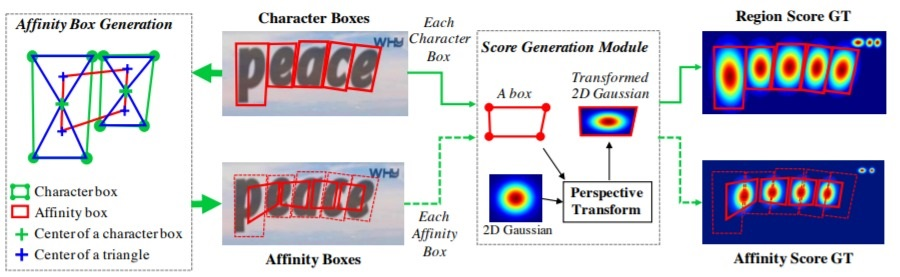
\includegraphics[width=0.9\linewidth]{img/baek}
	\caption{Wortdetektion}
	\label{fig:baek}
\end{figure}


Nach der Lokalisierung eines Kennzeichen und der daraus gewonnen Koordinaten, werden die gewonnen Informationen in EasyOCR weiterverarbeitet und mittels eines CRNN (Convolutional Recurrent Neural Network) Netzes bestehend aus drei Komponenten ausgelesen. Es handelt sich dabei um eine Feature Extraction, des Gesuchten Inputs mittels eines ResNets, um ein LSTM (Long-short term memory) Netz für das sequenzielle Labeling von Charakteren innerhalb eines Wortes. LSTM Netze eignen sich dabei besonders für die Verarbeitung sequenzieller Daten. Die dritte Komponente besteht aus einem CTC (connection temporal classification) Netz und ist für das Decoding der Outputs innerhalb des LSTM Netzes zuständig. \autocite[Vgl.][]{JaidedAI70}

Dieser Ansatz scheiterte jedoch, weil EasyOCR von Torch abhängt, Torch ein 64bit-Betriebssystem voraussetzt und Pi OS für den Raspberry Pi 3 zum Zeitpunkt der Projektdurchführung nur als 32bit-Version verfügbar war.
Die Alternative Lösung war Tesseract, eine OCR-Engine, die ursprünglich von Hewlett-Packard entwickelt wurde. Seit 2005 ist es Open-Source und von 2006 bis 2018 wurde es von Google weiterentwickelt. https://tesseract-ocr.github.io/docs/tesseracticdar2007.pdf %TODO

Tesseract bedient sich auch eines LSTM Netzes, benötigt jedoch kein 64Bit System. Bei der Umsetzung wird auf $Pytesseract$ und ein vortrainiertes englisches Modell der Texterkennung zurückgegriffen. \autocite[Vgl.][]{Tesserac98}
Dabei wird auch wieder auf ein Preprocessing gesetzt, dass das Bild in Graustufen konvertiert. Des Weiteren wird versucht mittels des Gauß-Verfahrens und gegebenen Filtern, Noise herauszufiltern. Dritter Schritt des Preprocessings ist das hervorhebenden der Kanten mittels der Konvertierung des Bildes in sogenannte $Blobs$, dabei handelt es sich um die Umwandlung eines Graubildes mittels eines festgelegten Schwellenwerts in Binäre Werte. \autocite[Vgl.][]{8974469} % Gehört das zu Tesseract oder ist das unser preprocessing?
Das Modell versucht, mittels Vektoren Linien auszumachen, auf denen sich die Schriftzüge befinden. Danach geht Tesseract dazu über, zeilenweise Wörter mittels der Bemessung von Abständen auszumachen und Wörter in Bounding-Boxes zu fassen. Die Erkennung der Texte geschieht über das vortrainierte englische LSTM Netz. Dieses weist bei der Umsetzung jedoch deutlich schlechtere Resultate auf als das zuvor verwendete CRNN (EasyOCR). Die Funktionalität und Genauigkeit beider Modelle wird in einem separaten Kapitel ausgewertet. %Ab hier Quarantäne, den Satz fass ich nicht an
%Da beide Modelle jedoch funktionieren ist es nicht von Nöten das schlechtere zu verwerfen, durch mehrere Versuche das Nummernschild zu lesen gelingt es beiden Modellen das richtige zu lesen. Lediglich die Halbwertszeit ist invers proportional zur Güte der Modelle. Somit ist man auch in der Lage mittels pytesseract die Nummernschild Erkennung durchzuführen und die Resultate mit einer White-list abzugleichen.

%Ende Quarantäne
%-> gelöscht, klarer Fall von Schweizer Grippe

\section{Evaluation der Pipeline}

Nach erfolgreichem Proof-of-Concept musste unter den technisch möglichen Varianten der Verarbeitungspipelines die beste ausgewählt werden. Hierzu wurde ein Notebook geschrieben, das die Pipeline in leicht abgewandelter Form für jedes Bild des gesammelten Datensatzes durchführt und das Ergebnis oder eventuelle Fehler in den einzelnen Bearbeitungsschritten festhält. Damit konnten verschiedene OCR-Verfahren untereinander verglichen werden. Ebenso war es möglich die bereits festgestellten Unterschiede in der Bearbeitungsgeschwindigkeit und Qualität von der Berechnung am Laptop gegenüber der Bearbeitung auf dem RasPi zu quantifizieren. Anhand der festgestellten Metriken können schlussendlich auch weiterführende Optimierungen vorgenommen und Fehlerquellen lokalisiert werden.

Die Kennzeichenerkennungspipeline besteht aus folgenden Schritten:

\begin{itemize}
\item Laden der kurz zuvor gespeicherten Datei
\item Preprocessing
\begin{itemize}
\item Umwandlung zu Graustufen
\item Bilateraler Filter
\item Canny-Algorithmus zu Kantenfindung
\item Douglas-Peucker-Algorithmus zur Erkennung von Rechtecken
\item Cropping
\end{itemize}
\item OCR mit vorgefertigter Lösung
\end{itemize}

\subsection{Cropping}
Bei 85 von 118 Bildern wurde eine Region als Kennzeichen identifiziert und freigestellt.
Diese ist nicht immer korrekt, es wurden neben Kennzeichen auch Fenster, Ziegelsteine und Straßenschilder freigestellt.
Das ist ein Problem, das durch die Vorschaltung von yolov3 verhindert werden könnte. 
Eine genauere Evaluation dieses Schrittes ist, ohne die Ergebnisse der nachgeschalteten OCR-Lösung zu berücksichtigen, wenig sinnvoll, weil der Bildausschnitt unvorhersehbare Folgen für das OCR-Ergebnis hat.


\subsection{OCR}
Beide OCR-Lösungen liefern ungenaue Ergebnisse. Die Plaketten zwischen den Blöcken der Kennzeichen werden oft als Zeichen interpretiert. Genauso wird zwischen den Blöcken manchmal ein Leerzeichen erkannt und manchmal nicht.
Bei einem genauen Vergleich dieser Ergebnisse mit einer Liste von erlaubten Kennzeichen würde daher sehr selten ein Treffer auftreten.

Aus diesem Grund wird stattdessen das Python-Paket \lstinline{thefuzz} verwendet, welches sich die Levenshtein-Distanz zu Nutze macht, um die Ähnlichkeit mehrerer Strings zu quantifizieren.
Um die Levenshtein-Distanz zwischen zwei Strings zu bestimmen, wird ein String zum Anderen umgeformt. Erlaubte Operationen sind dabei das Einfügen eines neuen Zeichens und das Entfernen eines bestehenden Zeichens.
Die minimal benötigte Anzahl dieser Operationen ist die Levenshtein-Distanz.

Hieraus wird ein prozentualer Wert abgeleitet, der die Genauigkeit der Erkennung widerspiegelt.
Für die finale Evaluation mit dieser Methode wurde ein Threshold von 45\% gewählt, um das gelesene Kennzeichen als richtig einzuordnen.

Mit easyOCR wurden 28 von 85 Kennzeichen richtig gelesen, mit Tesseract 17.
\begin{figure}[H]
		\centering
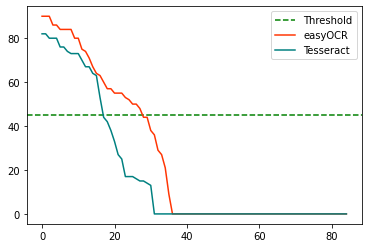
\includegraphics[width=8cm]{./img/evaluation_fuzzy_ratio.png}
\caption{Evaluation mit fuzzy ratio}
\end{figure}


Neben dem vollständigen Fuzzy Matching können mit der Funktion \lstinline{fuzz.partial_ratio()} auch Substrings berücksichtigt werden.
Das ist sinnvoll, um beispielsweise die Namen von Autohäusern aus den OCR-Ergebnissen herauszufiltern.
Mit dieser Methode (Threshold 45\%) liest easyOCR 31 von 85 Kennzeichen richtig, Tesseract 22. Dies entspricht 26\% bzw. 19\% der Ausgangsmenge von 118 Kennzeichen.
\begin{figure}[H]
		\centering
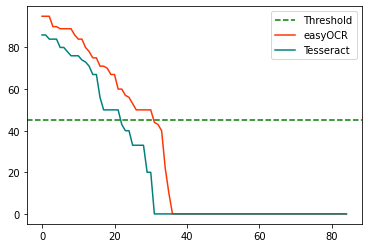
\includegraphics[width=8cm]{./img/evaluation_partial_ratio.png}
\caption{Evaluation mit partial ratio}
\end{figure}


Abgesehen von den bestehenden Methoden zum Vergleich mehrerer Strings wurde auch ein spezialisierter Ansatz entwickelt. Sowohl easyOCR als auch Tesseract haben die Schwäche, dass sie manchmal die Blöcke der Kennzeichen vertauschen. Um dieses Problem zu umgehen, wurde folgende, auf das vorliegende Problem spezialisierte, Funktion zur Evaluation entwickelt:

% TODO: Formatierung prüfen
\begin{lstlisting} 
def custom_match(read, label):	
	for x in label:
		if x not in read:
			return 0
	return 100
\end{lstlisting}     
% Bild dazu: eval_custom
Die Werte 0 und 100 dienen der einheitlichen Visualisierung. \lstinline{read} ist der Text, den die OCR-Lösung erkannt hat. \lstinline{label} ist das Label des jeweiligen Bildes in der Form \lstinline{OG AE 1337}. Die leerzeichengetrennten Teile des Labels werden durch Python in jeweils einzelnen Schleifendurchläufen behandelt.
Mit dieser Methode erzielt easyOCR 21 richtige Ergebnisse, Tesseract 5.
\begin{figure}[H]
		\centering
	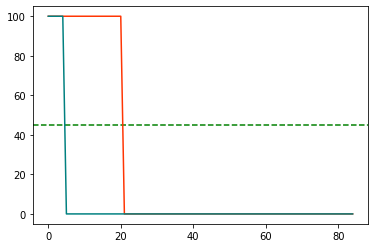
\includegraphics[width=8cm]{./img/evaluation_custom_matcher.png}
	\caption{Evaluation mit eigener Funktion}
\end{figure}


Es ist zu beachten, dass nicht alle im Vorigen Schritt freigestellten Bildsegmente auch wirklich Kennzeichen sind. Ein Mensch könnte an dieser Stelle also auch keine perfekte Leistung erreichen. 

\subsection{Laufzeit}

Für eine praktische Anwendung darf die Laufzeit der gesamten Pipeline nicht zu lang sein.
%Wenn die Laufzeit der Pipeline, also die Verzögerung zwischen der Aufnahme zweier Bilder \delta t ist,
%dann wird das 

Erstens sollte die Zeit zwischen dem Auftauchen des Autos vor der Kamera und dem ersten Scan konsistent sein,
zweitens kann die Pipeline im gleichen Zeitraum mehrmals ausgeführt werden und so trotz ungenauen Modellen gute Ergebnisse erzielen.
Die Laufzeit hängt direkt von der verwendeten Hardware ab.

Zur Evaluation wird die Dauer der einzelnen Schritte (Cropping und OCR) gemessen und zu Durchschnitten aggregiert. 

Auf dem selbst erstellten Datensatz wurde mit einem Lenovo Thinkpad T580 (Intel i7-8850U) für das Cropping durchschnittlich 1,37 Sekunden,
für die Texterkennung mit easyOCR 2,27 Sekunden und für die Bilderkennung mit Tesseract 2,67 Sekunden benötigt.
Das entspricht einer Gesamtlaufzeit von rund 4 Sekunden, also etwa 15 Bildern pro Minute.

Wird jedoch stattdessen ein Raspberry Pi 3 verwendet, steigt die Laufzeit auf durchschnittlich 14,87 Sekunden für das Cropping und 17,62 Sekunden für die Texterkennung mit Tesseract, also insgesamt 32,49 Sekunden.
EasyOCR wurde nicht evaluiert, weil es nicht mit der verwendeten Version von Pi OS kompatibel ist.

Beachtet man, dass das System im schlimmsten Fall kurz vor Ankunft des Fahrzeugs ein Bild aufnahm, so vergehen selbst bei einer direkten Erkennung etwa 60 Sekunden bis zur nächsten Aufnahme und Auswertung. 

\subsection{Zwischenfazit}
Geht man von der besten erreichten Erkennungsrate von 26\% aus, so beträgt der Erwartungswert der benötigten Erkennungsdurchläufe 100/26 = 3,84, welche wiederum 125 Sekunden benötigten. Dazu kommen durchschnittlich 0.5 * 32 Sekunden zur Beendigung der beim Eintreffen ablaufenden Schleife. Die Durchschnittliche Wartedauer beträgt also 141 Sekunden oder 2 Minuten und 21 Sekunden. 
\newline Natürlich ist hier zu beachten, dass beim Warten und der erneuten Bildverarbeitung das Bild ggf. nicht so stark vom vorherigen abweicht wie beim Datensatz und die gleichen Problembereiche hat. Die Erfahrungen im Praxistest auf der Straße lassen aber eher auf eine große Varianz der erkannten Flächen und Texte schließen, weshalb der Wert sich durchaus als Schätzung verwenden lässt.

Die durchschnittliche Wartedauer W bis zum Start der Öffnung lässt sich somit allgemein mit  Formel \ref{wartezeit} berechnen, wobei p die Erkennungswahrscheinlichkeit und t die Ausführungsdauer des Skripts darstellt.

\begin{equation}
	W=\frac{1}{p} * t + \frac{t}{2}
\label{wartezeit}
\end{equation}

% !TEX root =  master.tex
\chapter{Validierung}
Nach erfolgreichem Proof-of-Concept musste unter den technisch möglichen Varianden der Verarbeitungspipelines die beste ausgewählt werden. Hierzu wurde ein Skript geschrieben, dass die Pipeline in leicht abgewandelter Form für jedes Bild des gesammelten Datensatzes durchführt und das Ergebnis oder eventuelle Fehler in den einzelnen Bearbeitungsschritten festhält. Damit konnten verschiedene OCR-Verfahren untereinander verglichen werden. Ebenso war es möglich die bereits festgestellten Unterschiede in der Bearbeitungsgeschwindigkeit und Qualität von der Berechnung am Laptop gegenüber der Bearbeitung auf dem RasPi zu quantifizieren. Anhand der festgestellten Metriken konnten schlussendlich auch weiterführende Optimierungen vorgenommen und Fehlerquellen lokalisiert werden.
Abbildung #TODO veranschaulicht den Aufbau des Dataframes, in dem die Ergebnisse gespeichert wurden.


\chapter{Alternative Öffnungsmöglichkeiten}
Dieses Kapitel behandelt die Einbindung des Sprachassistenten, der Weboberfläche, des RFID-Moduls, des Ultraschallsensors und den praktischen Aufbau und Verkabelung aller Module.

\section{Sprachassistenten-Steuerung}
Zunächst wurde versucht den Sprachassisten Alexa von Amazon an den Raspberry Pi anzubinden. Die entsprechenden Bibliotheken konnten zwar installiert werden, auf der Developer-Oberfläche von Amazon erschienen allgemeine Fehlermeldungen die keinem konkreten Problem zuzuordnen waren. Die Verbindung zur Software auf dem Raspberry Pi konnte aber nachgewiesen werden, sodass wir von einer fehlerhaften Syntax der übertragenen Inhalte ausgehen, vermutlich durch Versionskonflikte.
Eine Alterative Lösung mit Google Home schien zunächst sehr vielversprechend, da Goolge in der Dokumentation ebenfalls einen Raspberry Pi als Einrichtungsbeispiel verwendet. Es stellte sich jedoch heraus, dass auch hier trotz orndungsgemäßem Befolgen der Anleitung keine Verbindung zustande kam. Die erhaltenen Fehlermeldungen ließen auf ein Paketproblem in der verwendeten Betriebssytemversion zu, die wird schlussendlich nicht lösen konnten. % TODO Anhang
Als Workaround wurde ein Alexa WiFi-Relais beschafft, das sich mit der App eines Drittanbieters (eWeLink) verbinden und dann in die Alexa-Umgebung integrieren lässt. Dieses Modul wurde nun so angeschlossen, dass es bei Aktivierung einen \ac{GPIO}-PIN mit 3.3V Spannung versorgt. Dieser Vorgang kann wiederum mit einer einfachen Schleife in einem Python Skript auf dem RasPi abgefragt werden und weitere Aktionen wie logging etc. ausgeführt werden. Prinzipiell wäre auch ein einfacherer, direkter Anschluss des Relais an den Garagentoröffner in Parallelschaltung möglich gewesen. Auf diesen wurde aber aus Kontroll- und Sicherheitsgründen verzichtet.

\section{Weboberfläche}
Da die Implementierung im Rahmen des Projekts auf einem Raspberry Pi stattfindet und Python bereits für viele Anwendungen innerhalb des Projekts verwendet wird, wird sich für das in Python geschriebene Webframework Flask entschieden. Dies hat den Vorteil, dass andere Komponenten, die bereits in Python geschrieben sind, direkt ohne Mehraufwand in die Weboberfläche integriert werden können.

Daher wird im Rahmen des Projekts für die Realisierung einer Weboberfläche eine einfache FlaskApp erstellt, die den üblichen Aufbau hat mit einer flaskapp.py, die die Weboberfläche steuert, und auf einzelne Templates, die wiederum in HTML geschrieben werden, zugreift. Hierbei wird in der flaskapp.py-Datei die Initialisierung der Weboberfläche sowie das Routing und dem Datentransfer zwischen den Seiten festgelegt sowie auch die Funktion, die die Garage öffnet. Als Templates die als Seite geladen werden, wird eines für die Startseite erstellt und eines für die Seite, auf der die Logs angezeigt werden sollen. Die Hauptseite, die bei Aufruf der Seite geladen wird, enthält einen Button, der mittels der in der flaskapp.py dafür festgelegten Funktion die SmartGarage öffnet und einen Eintrag in der Logs-Datei erstellt. Des Weiteren enthält diese Seite die Information ob in der Garage ein Fahrzeug steht, oder nicht. Dies geschieht über die Ultraschallmessung, wie bereits zuvor erläutert. Ebenfalls wird von dieser Seite aus auf die Logs-Seite verlinkt. Die Logs-Seite bezieht die Daten aus der Logs-Datei und gibt diese auf der Weboberfläche aus, wodurch der Besitzer der Garage die geloggten Öffnungen einsehen kann.

\section{RFID}

Die Implementierung eines RFID-Systems in der SmartGarage bietet eine weitere Möglichkeit die Garage zu öffnen. Für das Projekt wurde daher ein RFID-RC522 Modul an den Raspberry Pi angeschlossen, welches als Lesegerät Transponder auslesen kann. Angesteuert vom Raspberry Pi wird das Modul mittels der GPIO-Ports ähnlich wie beispielsweise bereits dem Ultraschallsensors. Das Auslesen wird dann mit Hilfe eines Python-Skripts gesteuert und mit einer Whitelist abgeglichen.
Trotz der komplexen Technik gelang der Anschluss dank eines online verfügbaren Tutorials problemlos.\autocite[Vgl.][]{tutorialrfikd}
Als Transponder kann im Projekt jede beschreibbare RFID-Karte oder RFID-Chipkarte verwendet werden, solange diese die vorausgesetzte Frequenz von 13,56MHz unterstützt. Im Projekt wird hierfür eine RFID-Karte, die nicht mit dem richtigen Code beschriftet ist, als Beispiel für eine fehlerhafte Identifikation verwendet. 
Die großen Vorteile der RFID-Öffnungsmöglichkeit gegenüber z.B. einem Schlüssel sind die Protokollierbarkeit und die einfache und kostengünstige Sperrung falls ein Transponder geklaut oder verloren wird. In diesem Fall genügt es, den entsprechenden Eintrag aus der Whitelist zu entfernen. 


\section{Ultraschallsensor}
TODO voherigen Teil aufsplitten, Quelle

\section{Öffnungssimulation}
Um die Betätigung des Handsenders bei der Entwicklung simulieren und Testen zu können, wurde statt dem Relais zunächst eine LED an die GPIO-Pins des RasPi angeschlossen. Da die Lichtverhältnisse manchmal schwierig waren, wurde zusätzlich ein sogenannter aktiven Summer eingesetzt. Dieser erklingt dann zum Beispiel, wenn der richtige RFID Chip an das Lesegerät gehalten wird und somit die Garage geöffnet oder geschlossen wird. Dabei handelt es sich um einen Oszillator der, wird er einer gewissen Spannung untersetzt, anfängt zu Vibrieren und damit ein Ton erzeugt. Ausgeführt und koordiniert wird der Buzzer über ein Simples Python Skript das mittels der Bibliothek GPIO (General-Purpose Input/Output) in der Lage ist den Buzzer an oder auszuschalten. Dabei wird durch einen definierten Port, in diesem Fall „Port 4“, mittels einer $for$ Schleife die Spannung je nach $positivem$ oder $negativem$ Signal Ton koordiniert und eine andere Tonsequenz abgespielt.

Zu Präsentationszwecken wurde der Code zum Aktivieren der LED bzw. des Buzzers dann durch einen anderen ersetzt, der per SSH auf einen zweiten Raspberry Pi zugreift und dort ein Video eines öffnenden und schließenden Garagentors abspielt.
Dabei wird lokal eine Binärvariable geändert um den Zustand des Garagentors (offen oder geschlossen) speichert und das richtige Video auswählt.
Jedoch funktioniert diese Lösung nicht ganz zuverlässig, da nach jedem Zugriff das Video des vorherigen Versuchs trotz geschlossener SSH-Verbindung offen bleibt. 


\section{Steckplan}

Auf Abbildung \ref{Steckplansm} ist die schlussendlich verwendete Steckung abgebildet. Hierbei war zu beachten, dass die im Internet verfügbaren Anleitungen und Tutorials nicht unbedingt miteinander kompatibel sind und einige \ac{GPIO}-Pins von mehreren Vorlagen verwendet werden. Hier muss demetsprechend ein anderer freier Pin mit gleicher I/O-Funktion gefunden werden und der Code angepasst werden. Außerdem ist die Spannung zwingend zu beachten. Manche Module, wie der Ultraschallsensor, benötigen eine Spannung von 5V, andere nur 3.3V. Die GPIO-Pins des Raspberry Pi, sind auf 3.3V ausgelegt und nicht vor Überspannug geschützt. Ein versehentliches Verbinden der beiden Spannungsnetze kann zu irreperablen Hardwareschäden führen. Deshalb wurde beispielsweie am Ultraschallsensor ein Spannungsteiler eingebaut.

Der zur Steckung gehörige elektrische Schaltplan findet sich in Anhang \ref{Schaltplan}.
Auf Abbild \ref{Aufbau1} ist der Aufbau in der Praxis abgebildet. Das Objekt rechts auf dem Bild ist ein 4G-Router, der aufgrund der schlechten Internetverbindung bei Gruppenarbeiten vor Ort benötigt wurde.
Weitere Bilder des Versuchsaufbaus in Anhang \ref{Aufbauanhang}
\begin{figure}[H]
	\centering 
	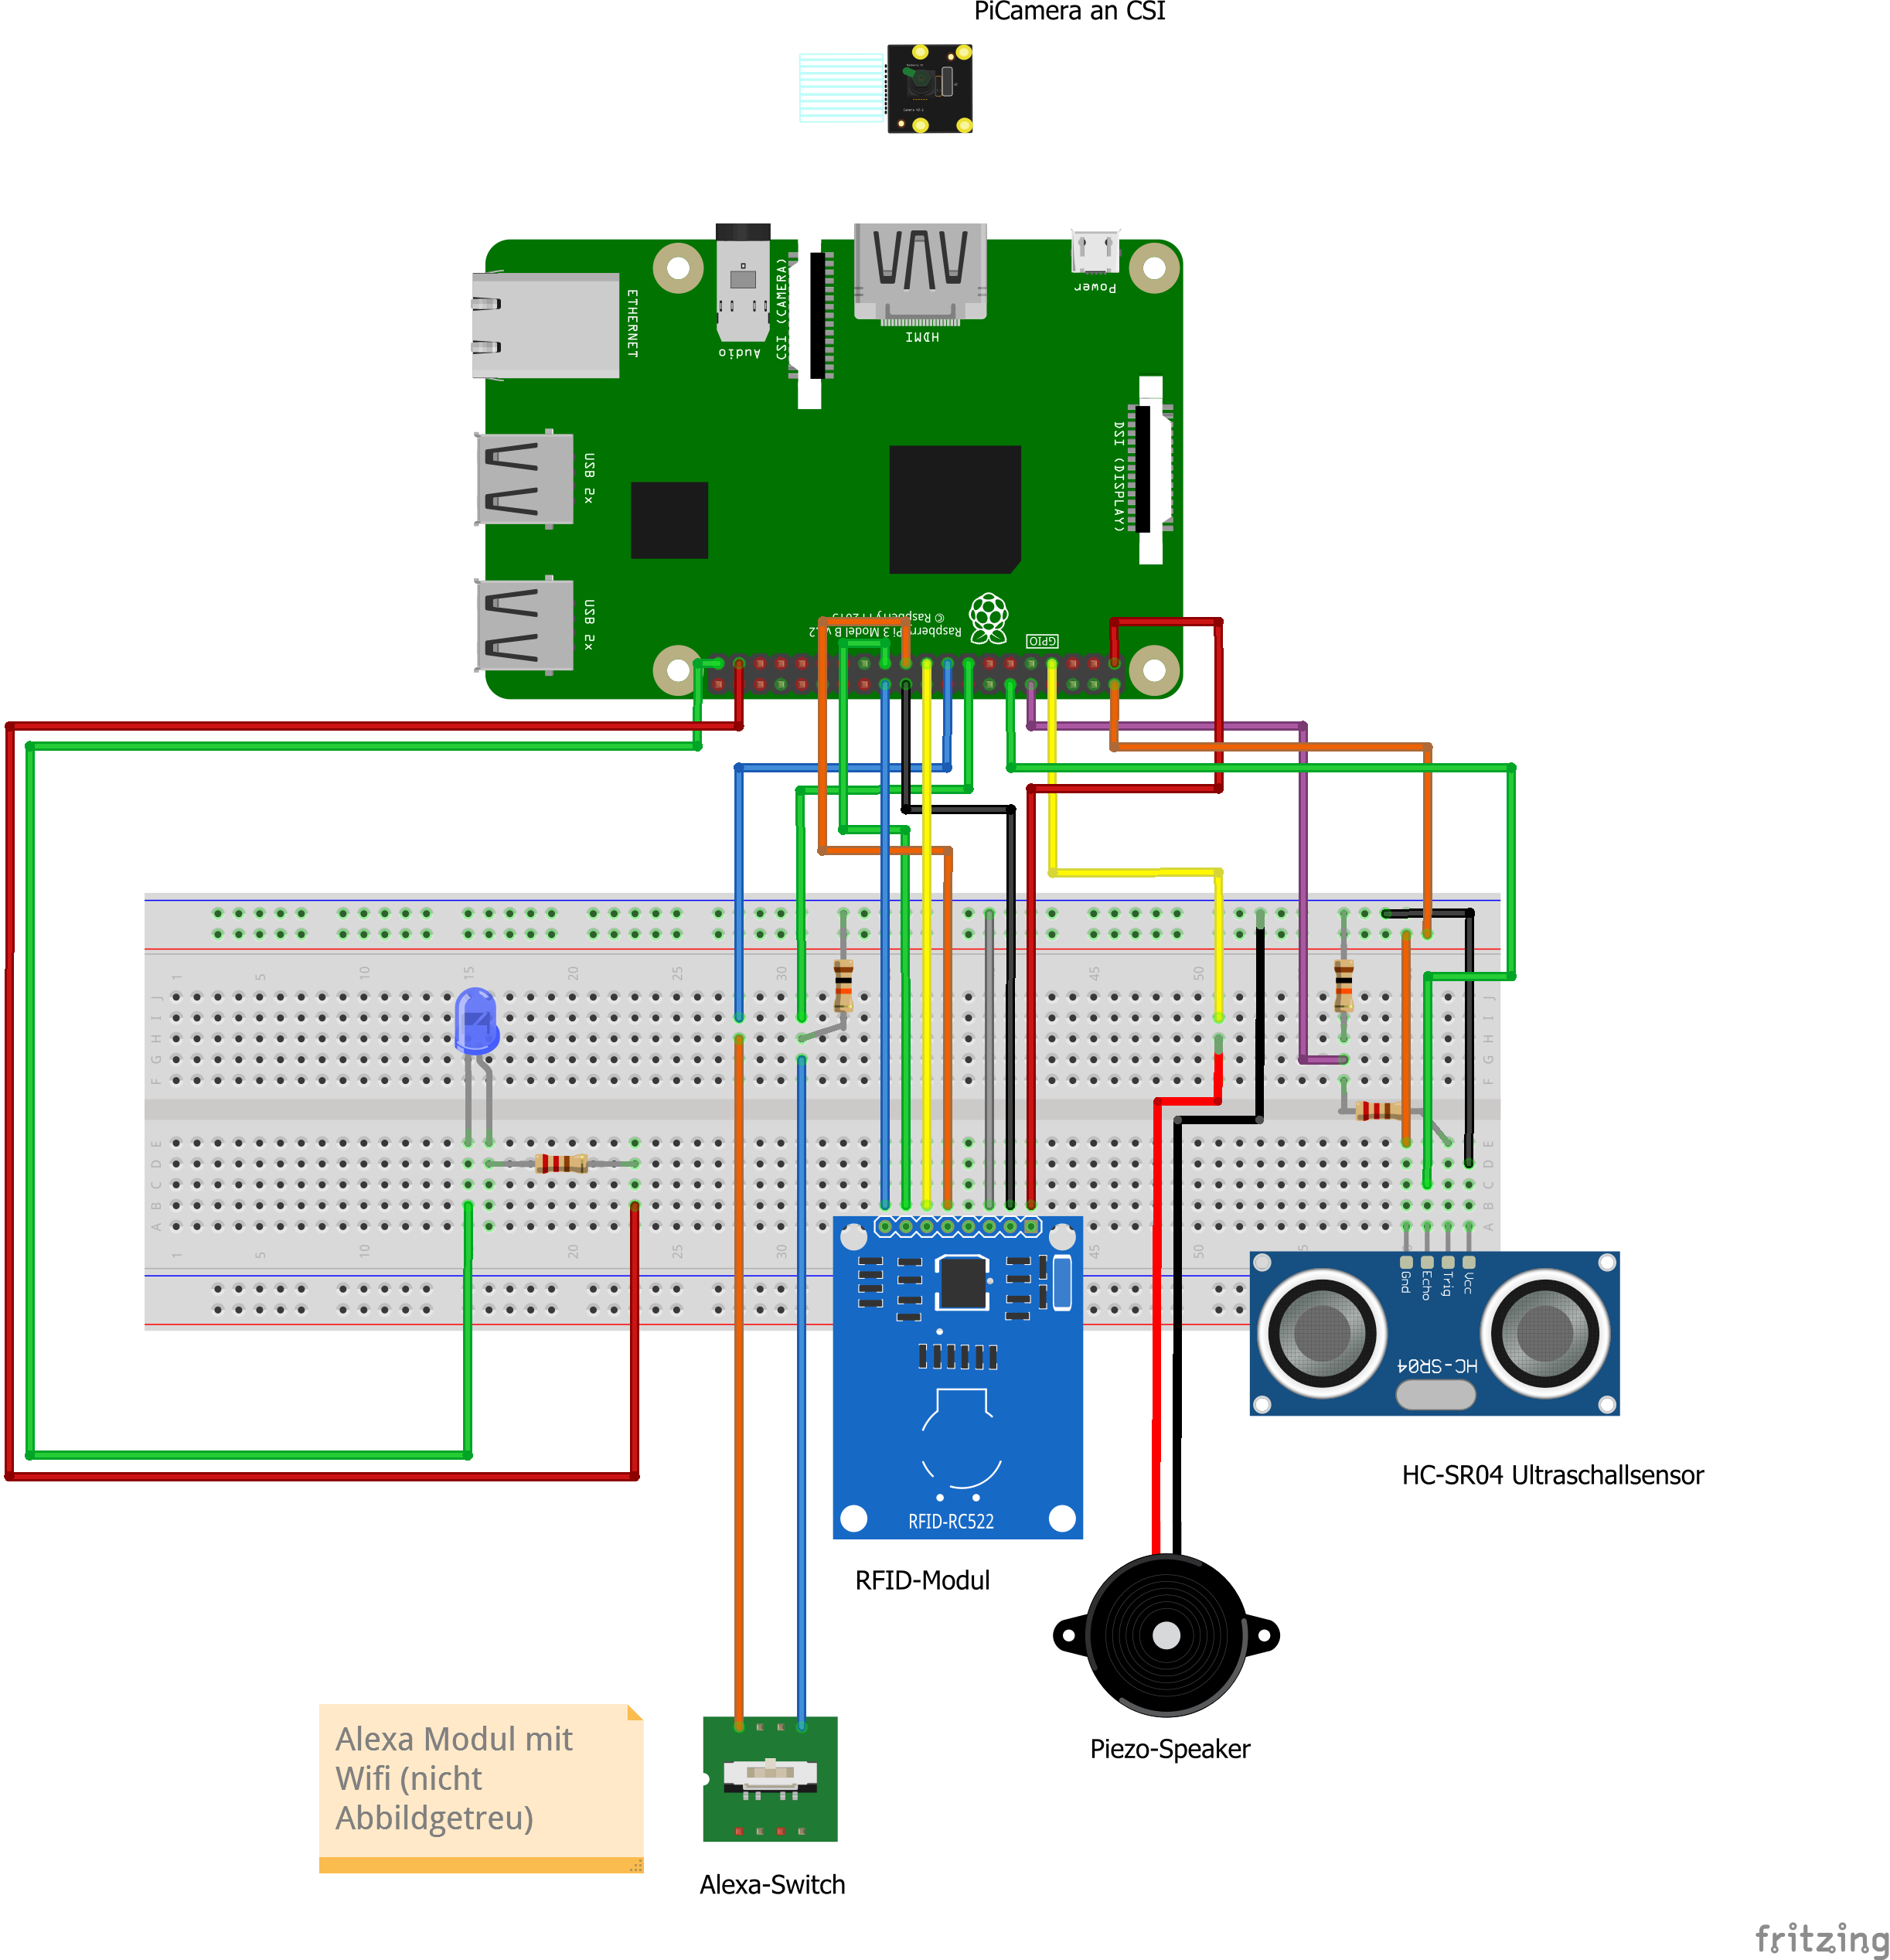
\includegraphics[scale=0.5]{\imagedir/SmartGarage.png}
	\captionsetup{format=hang}
	\caption[Steckplan]{\label{Steckplansm}Steckplan der gesamten Hardware \\Quelle: Eigene Darstellung}
\end{figure}
\begin{figure}
	\centering 
	\label{}
	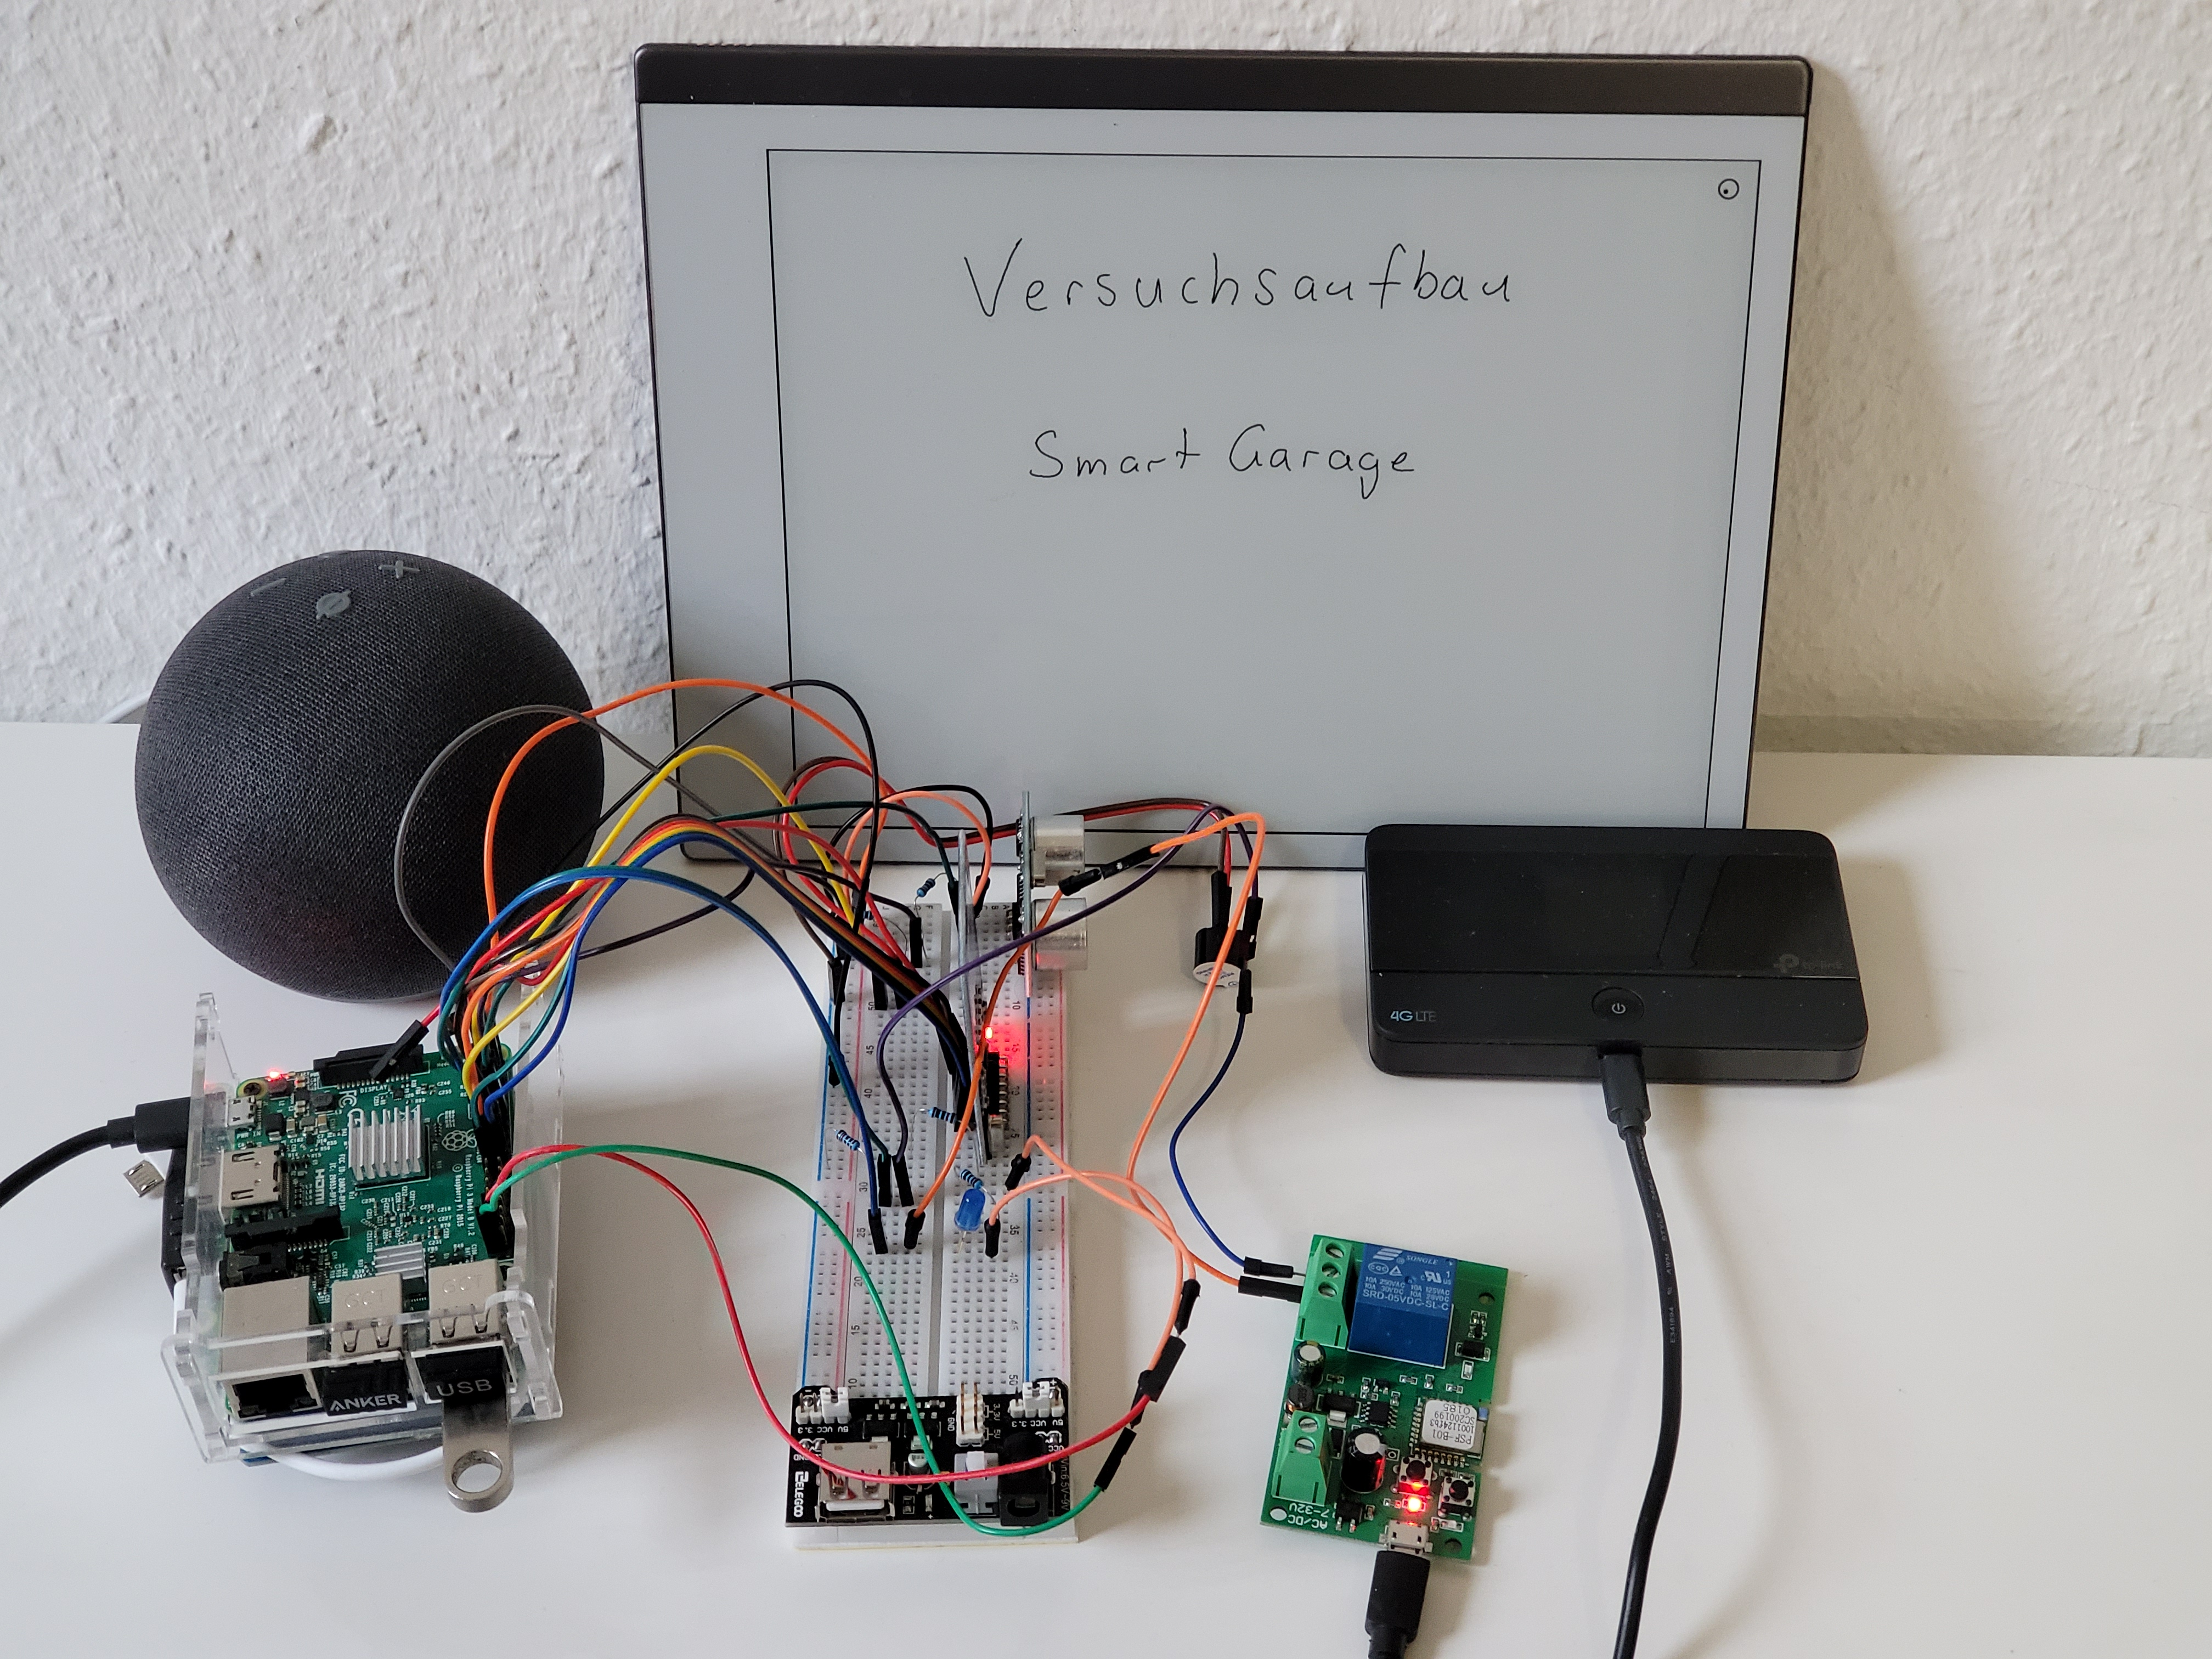
\includegraphics[scale=0.08]{\imagedir/Foto (7).jpg}
	\captionsetup{format=hang}
	\caption[Versuchsaufbau]{\label{Aufbau1}Fertiger Aufbau aller Module\\Quelle: Eigene Darstellung}
\end{figure}
\chapter{Risiken und Limitierungen}

Mehrere problematische Punkte konnten innerhalb der relativ kurzen Projektlaufzeit noch nicht ausreichend adressiert werden. Sie wurden aber erfasst und in diesem kurzen Abschnitt notiert.

Zum einen hat die verwendete Software noch Schwierigkeiten mit Störungen durch Fahrzeug- und Kennzeichenhalterbeschriftungen und deutsche Umlaute, die in manchen Kennzeichen vorhanden sind, können noch nicht erkannt werden. Dies war auf den erfassten Testdaten in Mannheim/Heidelberg nicht nicht problematisch, wird es aber für andere Regionen sein.
Zum anderen ergeben sich durch die optische Erkennung naturgemäß etliche Probleme bei erschwerten Sichtverhältnissen wie Schnee, Regen, Dunkelheit oder schlicht verschmutzten Kennzeichen. 

Ein weiterer bedeutender Punkt ist die mangelnde Sicherheit des Systems. Da die Öffnung des Garagentors nur durch das Kennzeichen geschieht, ist das Missbrauchs-bzw. Einbruchspotenzial groß. Im schlimmsten Fall reicht ein bedrucktes DIN-A4 Blatt mit dem richtigen Kennzeichen um die Garage zu öffnen. Auch Hackerangriffe sind prinzipiell möglich.

Ebenfalls sollte bei der Installation der Datenschutz beachtet werden. So ist es nicht erlaubt öffenliche Bereiche zu filmen.

Eine Messung des Stromverbrauchs hat nicht stattgefunden, dementsprechend kann auch keine Aussage über die laufenden Betriebskosten des RasPi mit allen Modulen und der Luxonis-Kamera getätigt werden.

\chapter{Wirtschaftliche Aspekte}
Auch wenn die technische Konzeption und Umsetzung im Mittelpunkt dieser Arbeit stehen, soll aufgrund der Ausrichtung des Studiengangs hier auch kurz auf einige betriebswirtschaftliche Aspekte des Projekts eingegangen werden.\subparagraph*{Entwicklungskosten}
   \newline
Zeitaufwand pro Teammitglied

\begin{tabular}[h]{lcr}
2x Projektkonzeption/Kick-Off online 2 Stunden \\
3x Workshops a 12 Stunden\\
2x Workshop a 8 Stunden\\
1x Praxistest 4 Stunden\\
1x Abschluss-Workshop a 24 Stunden \\
8 Stunden Ausarbeitung Projektbericht / Dokumentation\\
\end{tabular} \newline

Bei einem angenommenen Stundenlohn von 15€, der für Werkstudenten mit vergleichbaren Kenntnissen angemessen ist, ergeben sich bei den aufsummierten 368 Mannstunden geschätzte kalkulatorische Entwicklungskosten von 5520€
\subparagraph*{Materialkosten} in Euro, inkl. Versand  \newline 

\begin{tabular}[h]{lcr}
Raspberry Pi 3	&   39,95 \autocite{Pi3b} \newline \\
RFID-Modul RC552 &		5,00\autocite{RFID} \newline\\
Ultraschallmodul	&  8,94\autocite{SR04} \newline \\
Amazon Alexa Wifi Modul & 13,99\autocite{eWe}	\\
OAK-D Kamera & 185,51 \autocite{eWe} \\
\textbf{Summe}			&	\textbf{253,39}
\end{tabular} \newline


Die geschätzte Installationszeit pro Einheit für Verkabelung des Kameramoduls und des RasPi, Befestigung des RFID-Sensors, Ausrichtung der Kamera und Tests beträgt für einen geübten Elektriker ca. 4 Stunden.
Bei einem angenommenen Kosten von 60€/Stunde wären dies 240€ (ohne Anfahrt). Der Verkaufspreis inklusive Installation müsste also mindestens bei knapp 500€ liegen, um einen Deckungskostenbeitrag zu erzielen und die Entwicklungskosten von 5520€ zu decken.





% Fazit und Ausblick
% !TEX root =  master.tex
\chapter{Zusammenfassung}

\nocite{*}

Dieses Kapitel enthält die Zusammenfassung der Arbeit mit Fazit und Ausblick.

\section{Fazit}

...

\section{Ausblick}

...


%%%%%%%%%%%%%%%%%%%%%%%%%%%%%%%%%%%

%%%%%%%%%%%%%%%%%%%%%%%%%%%%%%%%%%%
% ANHÄNGE
%
% @stud: einzelne Anhänge bearbeiten und eigene Anhänge hier einfügen 
%        die nachfolgenden Zeilen deaktivieren, wenn keine Anhänge verwendet werden
%
\initializeAppendix
% !TEX root =  master.tex
\chapter{Ablaufplan}
\begin{figure}[H]
	\centering 
	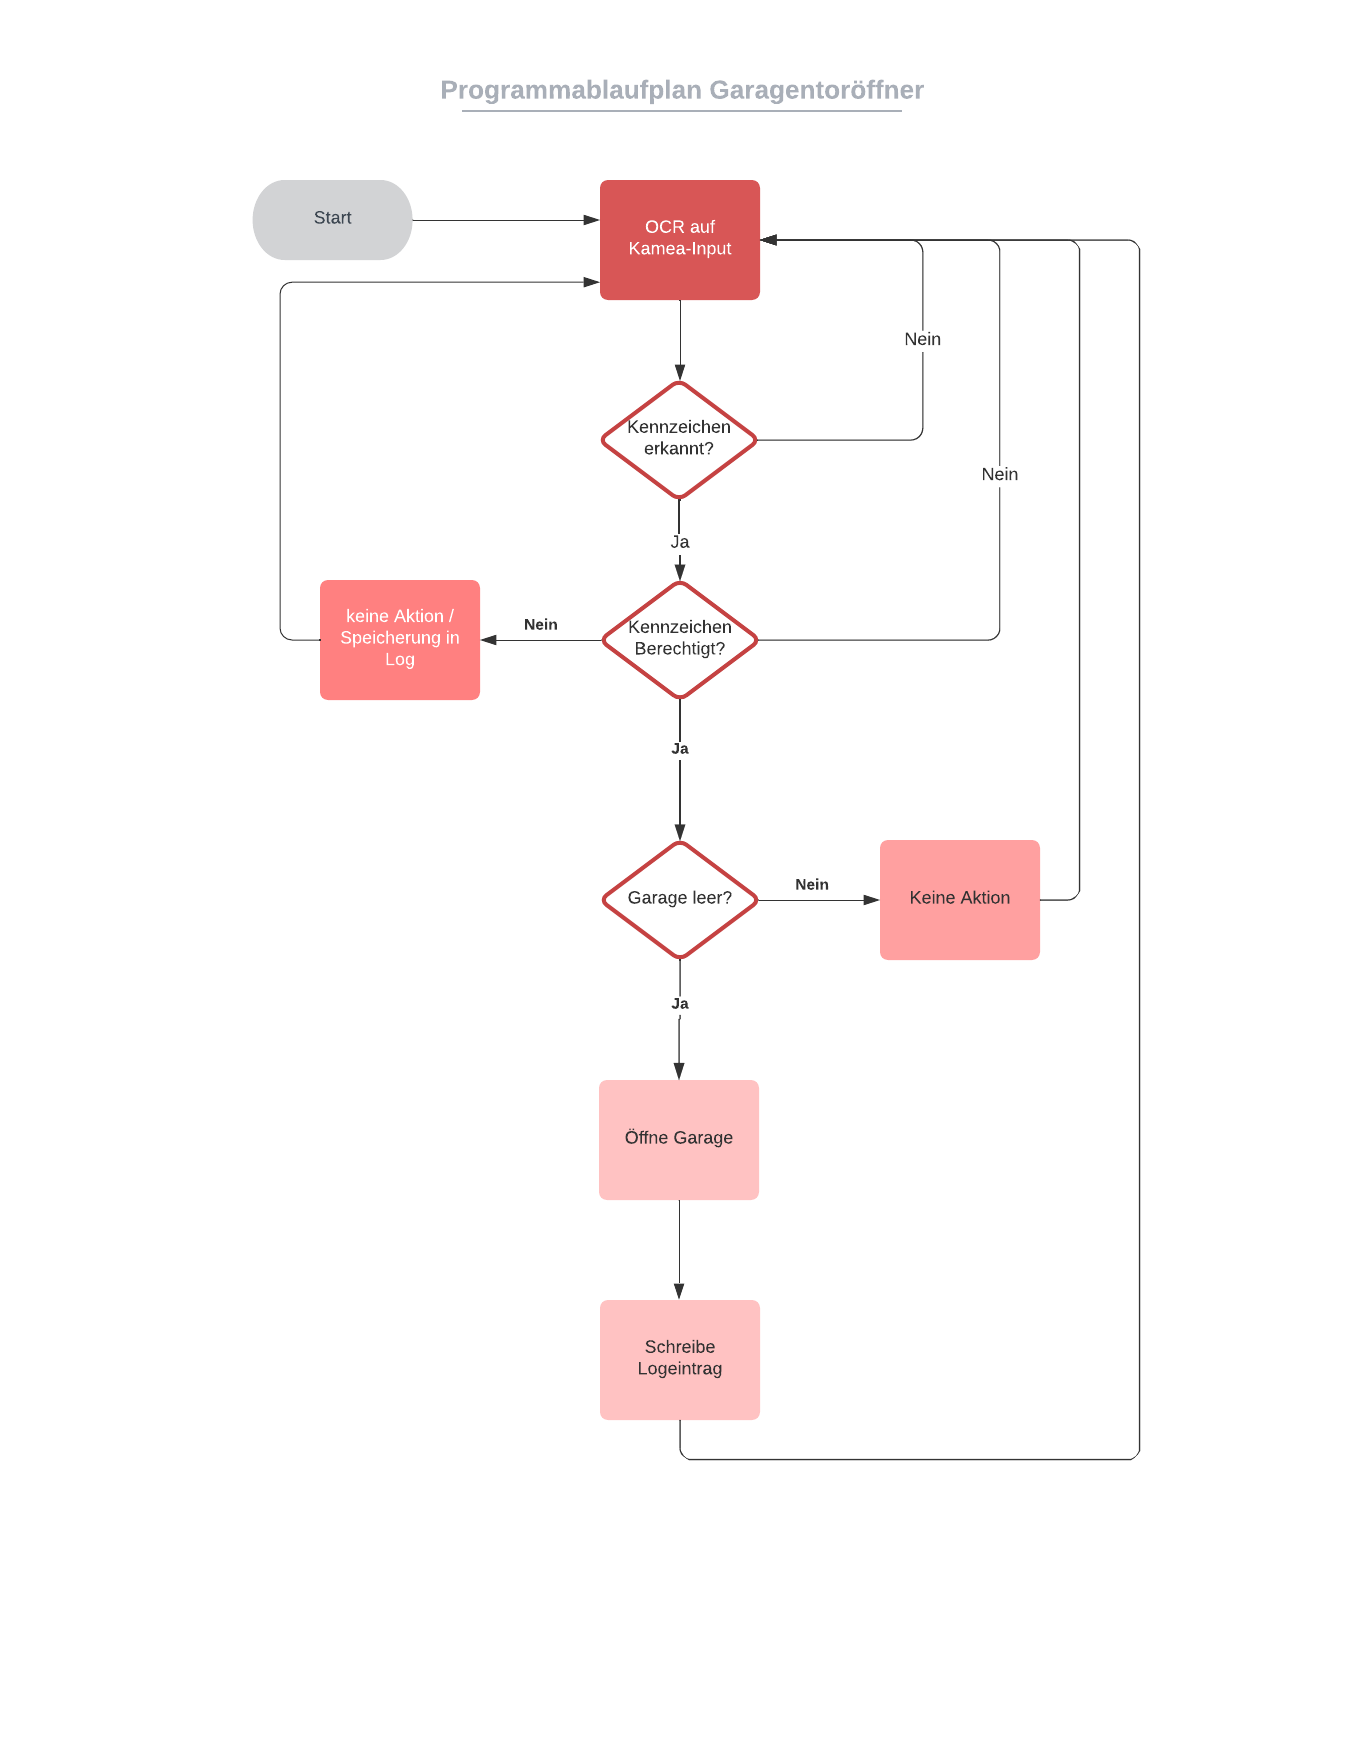
\includegraphics[scale=0.75]{\imagedir/Programmablaufplan.png}
	\captionsetup{format=hang}
	\caption[Programmablauf]{\label{Ablaufplan}Ablauf der Kennzeichenerkennungs-Schleife \\Quelle: Eigene Darstellung}
\end{figure}
\chapter{Schaltplan}
\begin{figure}[H]
	\centering
	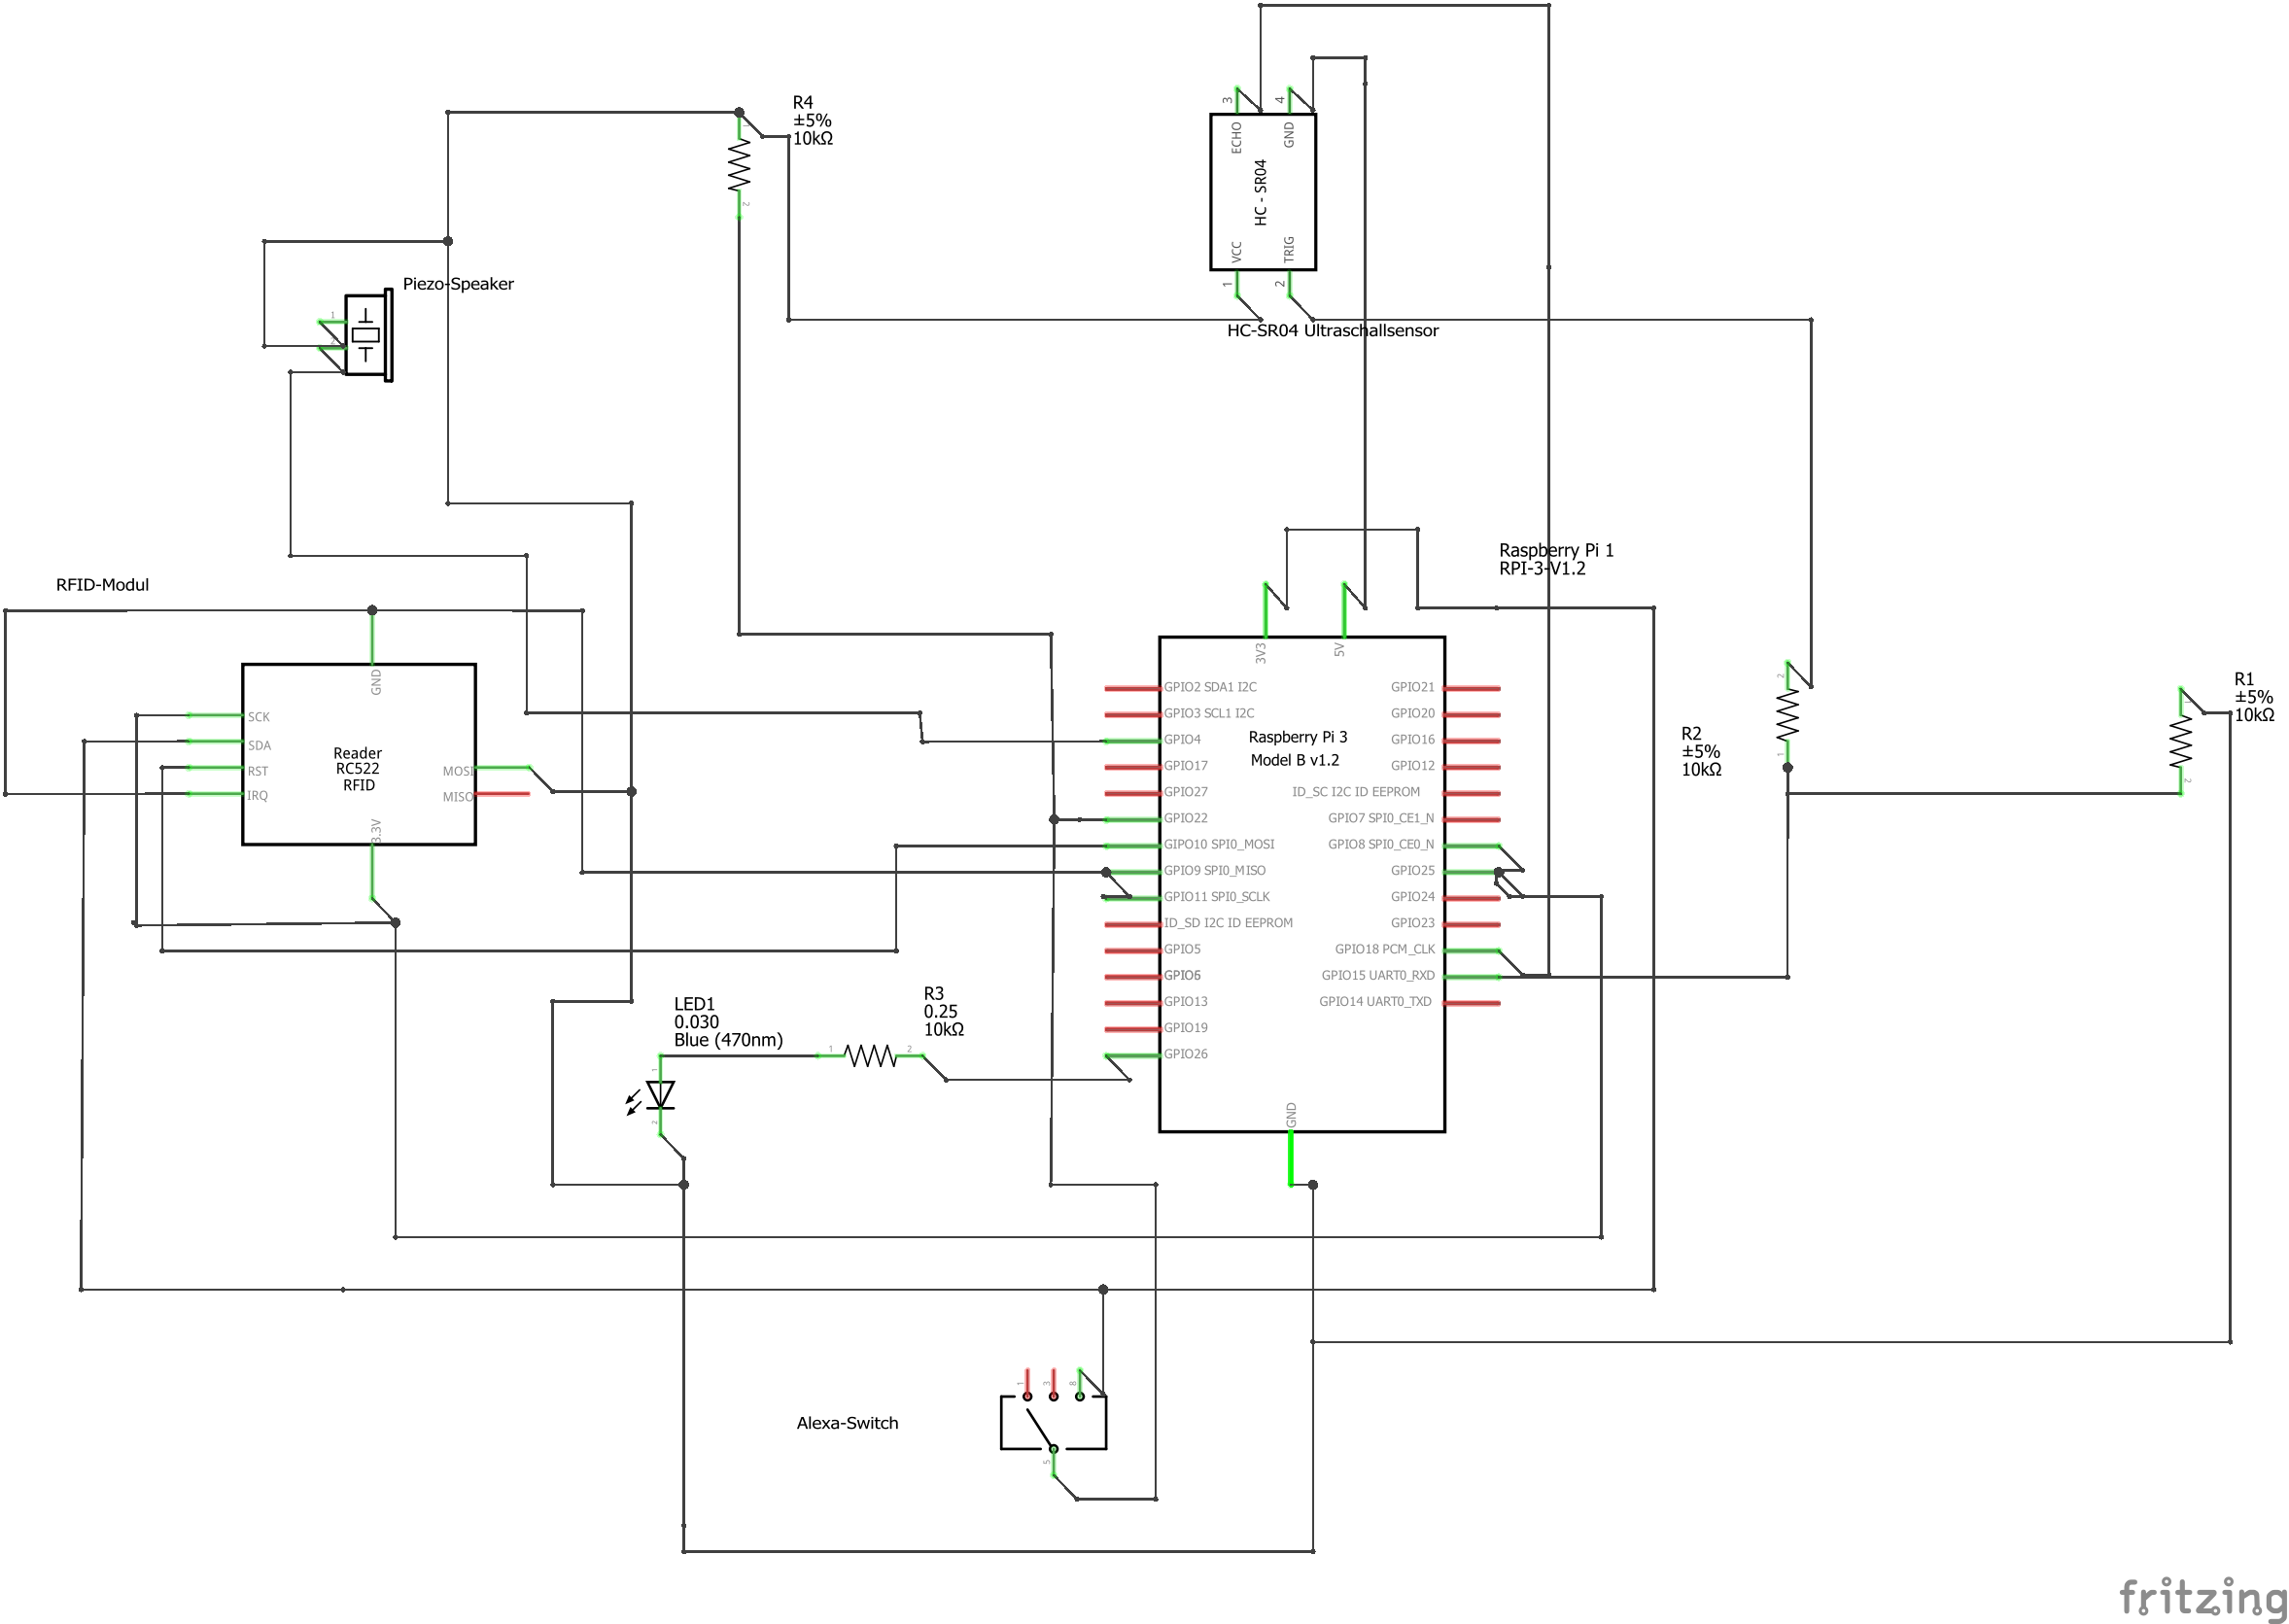
\includegraphics[width=1\linewidth]{img/SmartGarage_Schaltplan}
	\caption[Schaltplan]{Finaler Schaltplan aller Bauteile \\ Quelle: Eigene Darstellung}
	\label{Schaltplan}
\end{figure}
\chapter{Steckplan}
\begin{figure}[H]
	\centering 
	\label{Steckplan}
	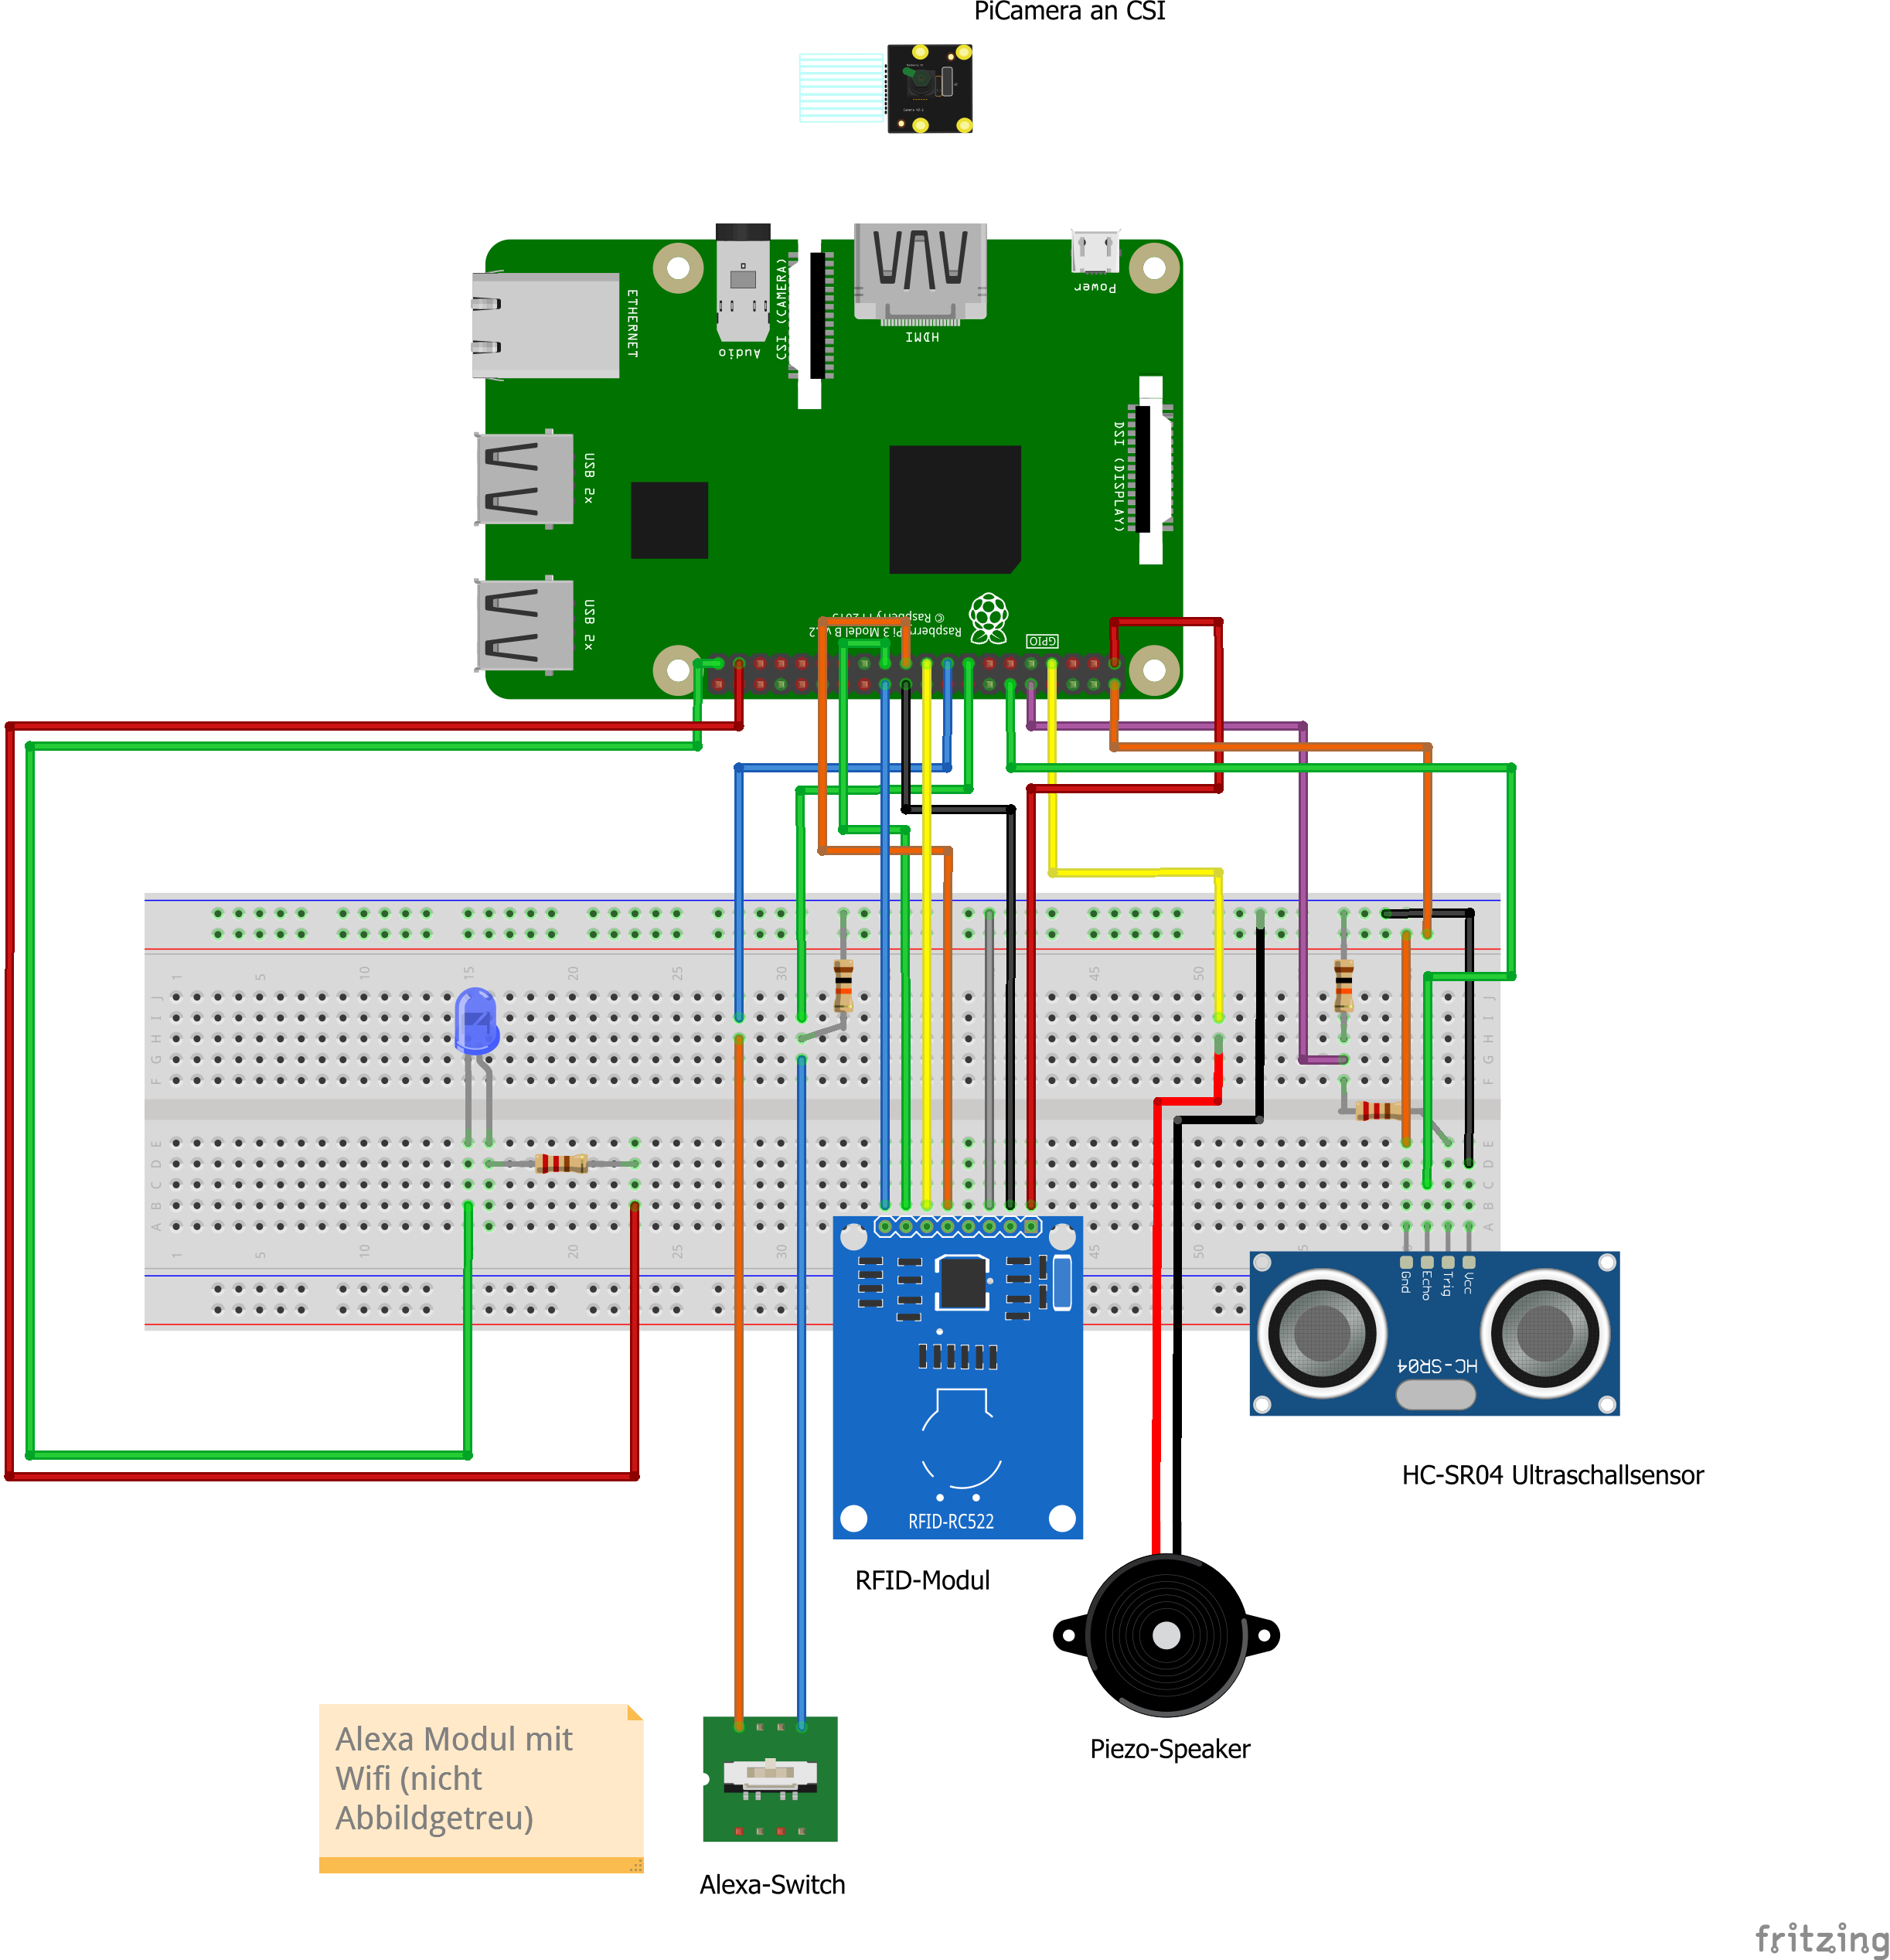
\includegraphics[scale=0.8]{\imagedir/SmartGarage.png}
	\captionsetup{format=hang}
	\caption[Steckplan groß]{Steckplan der gesamten Hardware \\Quelle: Eigene Darstellung}
\end{figure}
\chapter{Versuchsaufbau}
\begin{figure}[h]
	\centering 
	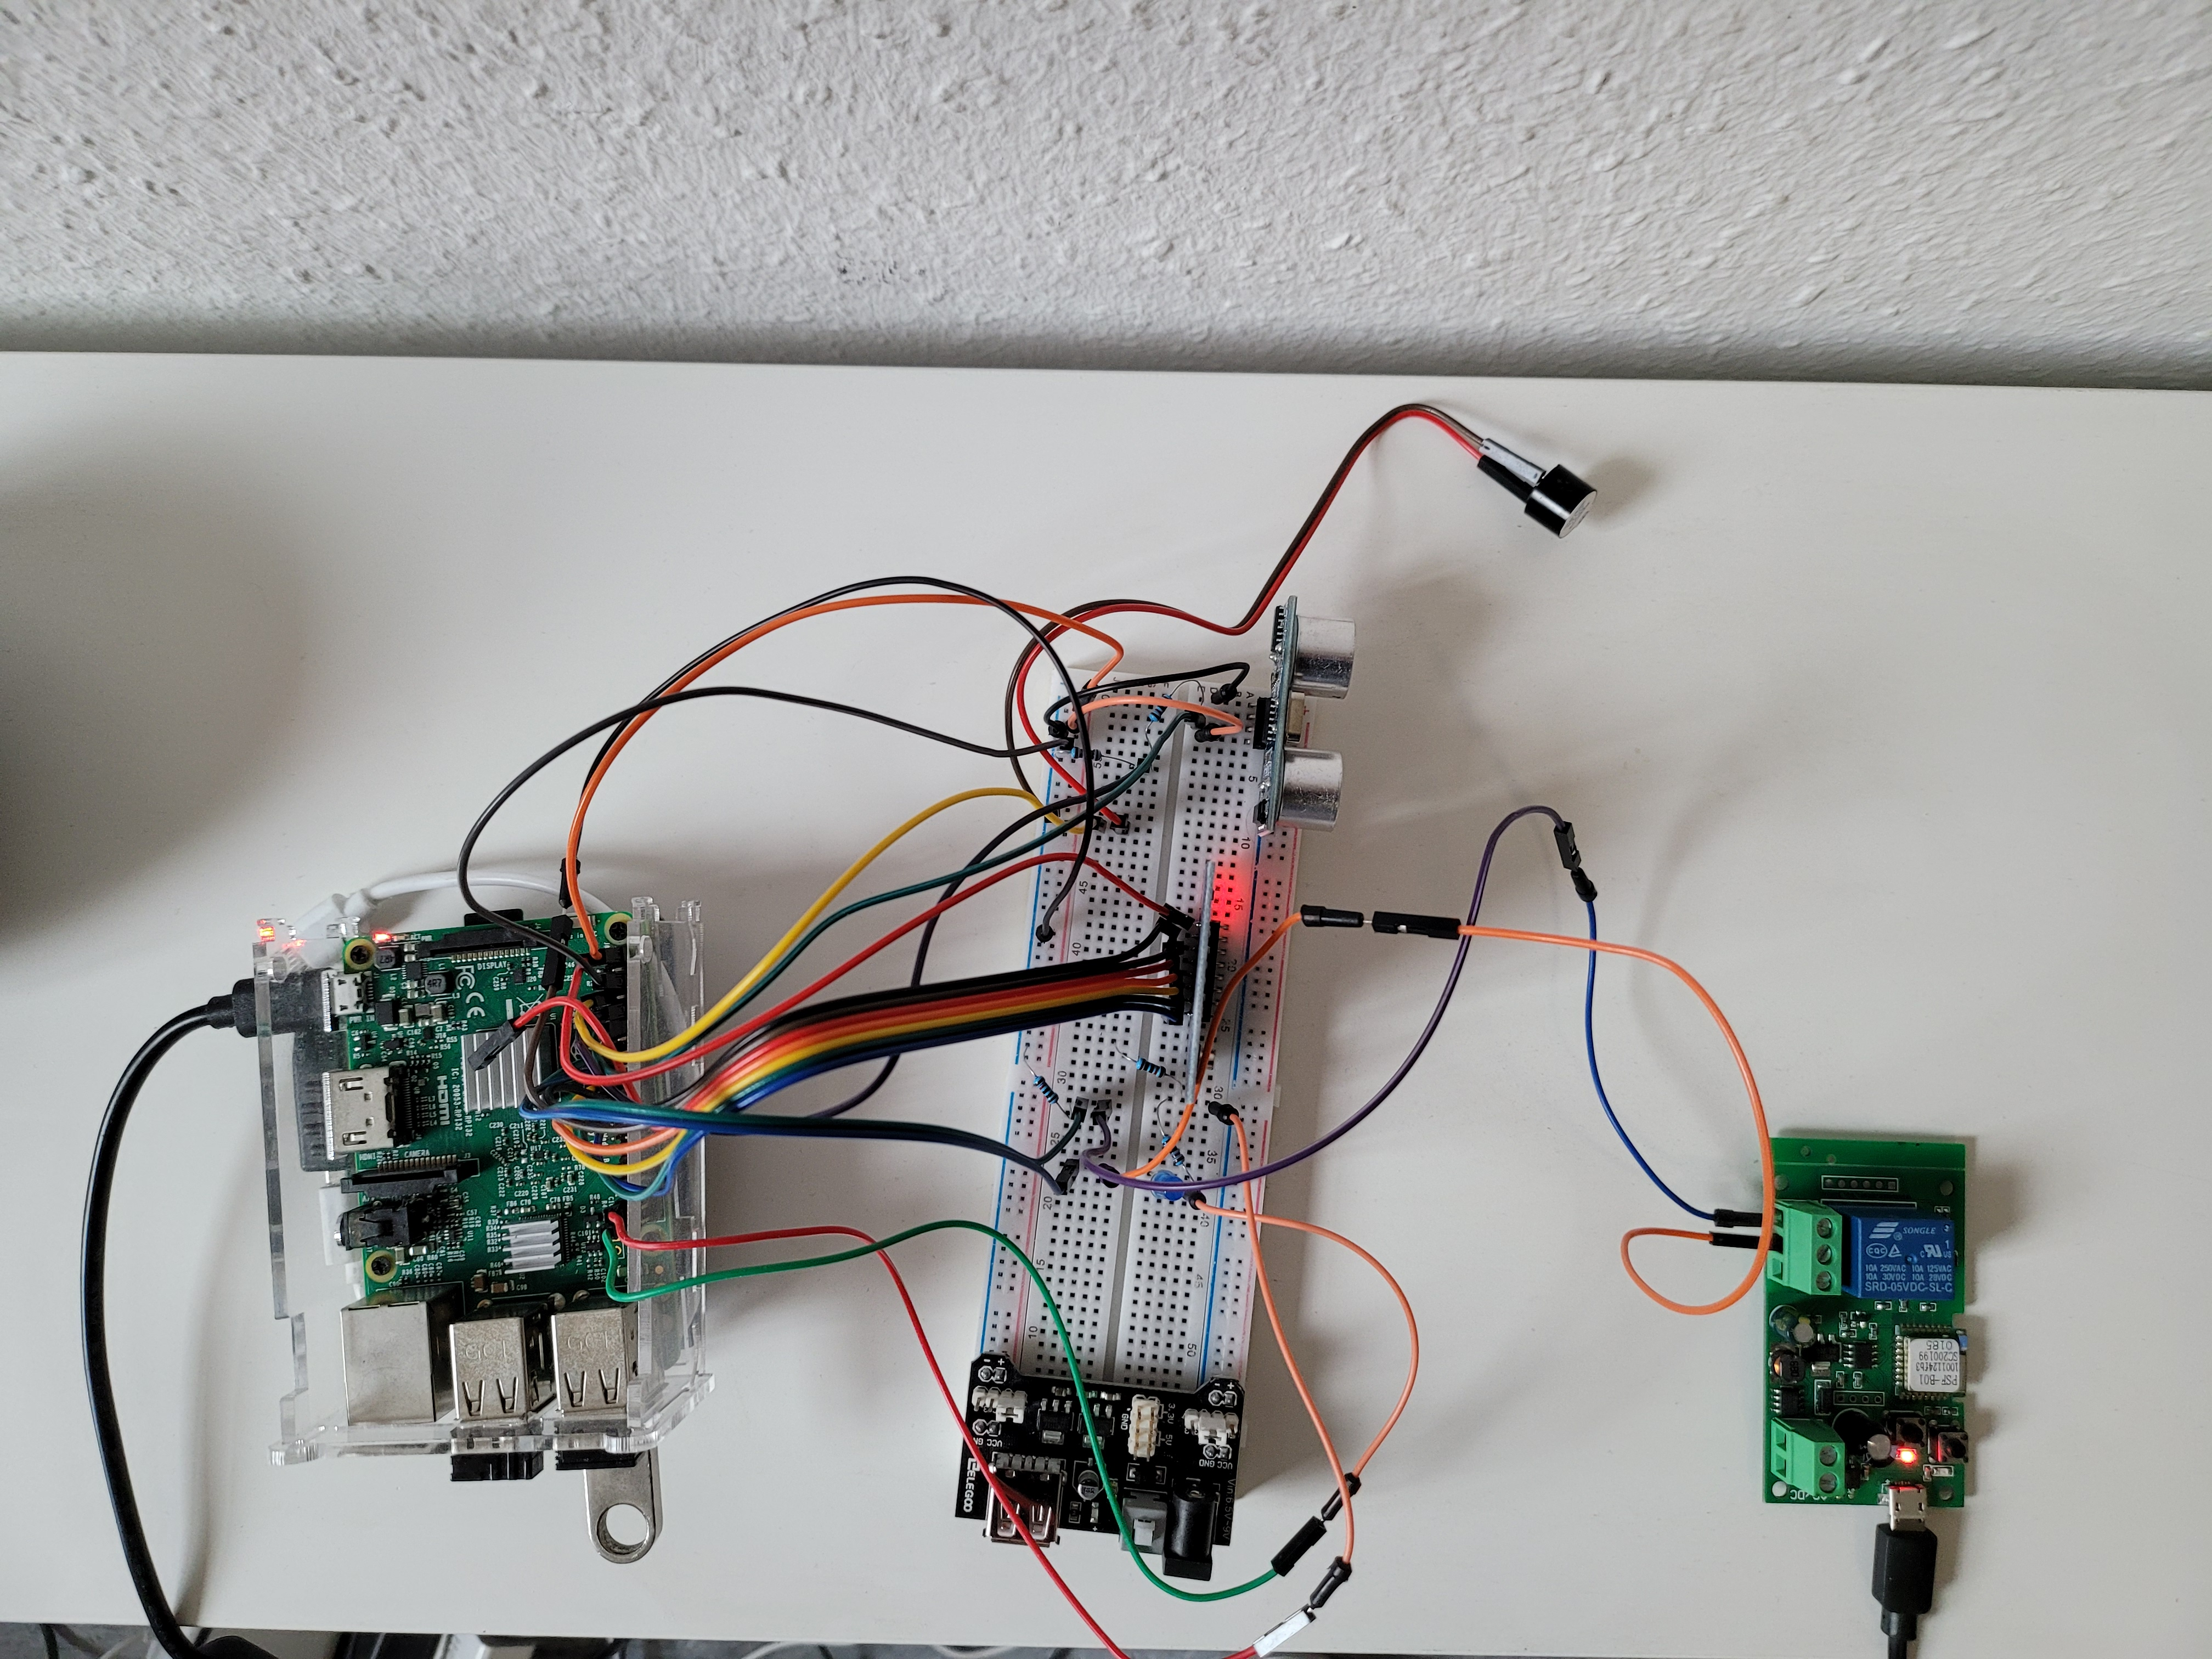
\includegraphics[scale=0.08]{\imagedir/Foto (1).jpg}
	\captionsetup{format=hang}
	\caption[Foto Aufbau 1]{\label{}Raspberry Pi, Breadboard und Alexa-Modul\\Quelle: Eigene Darstellung}
\end{figure}
\begin{figure}[H]
	\centering 
	\label{Aufbau2}
	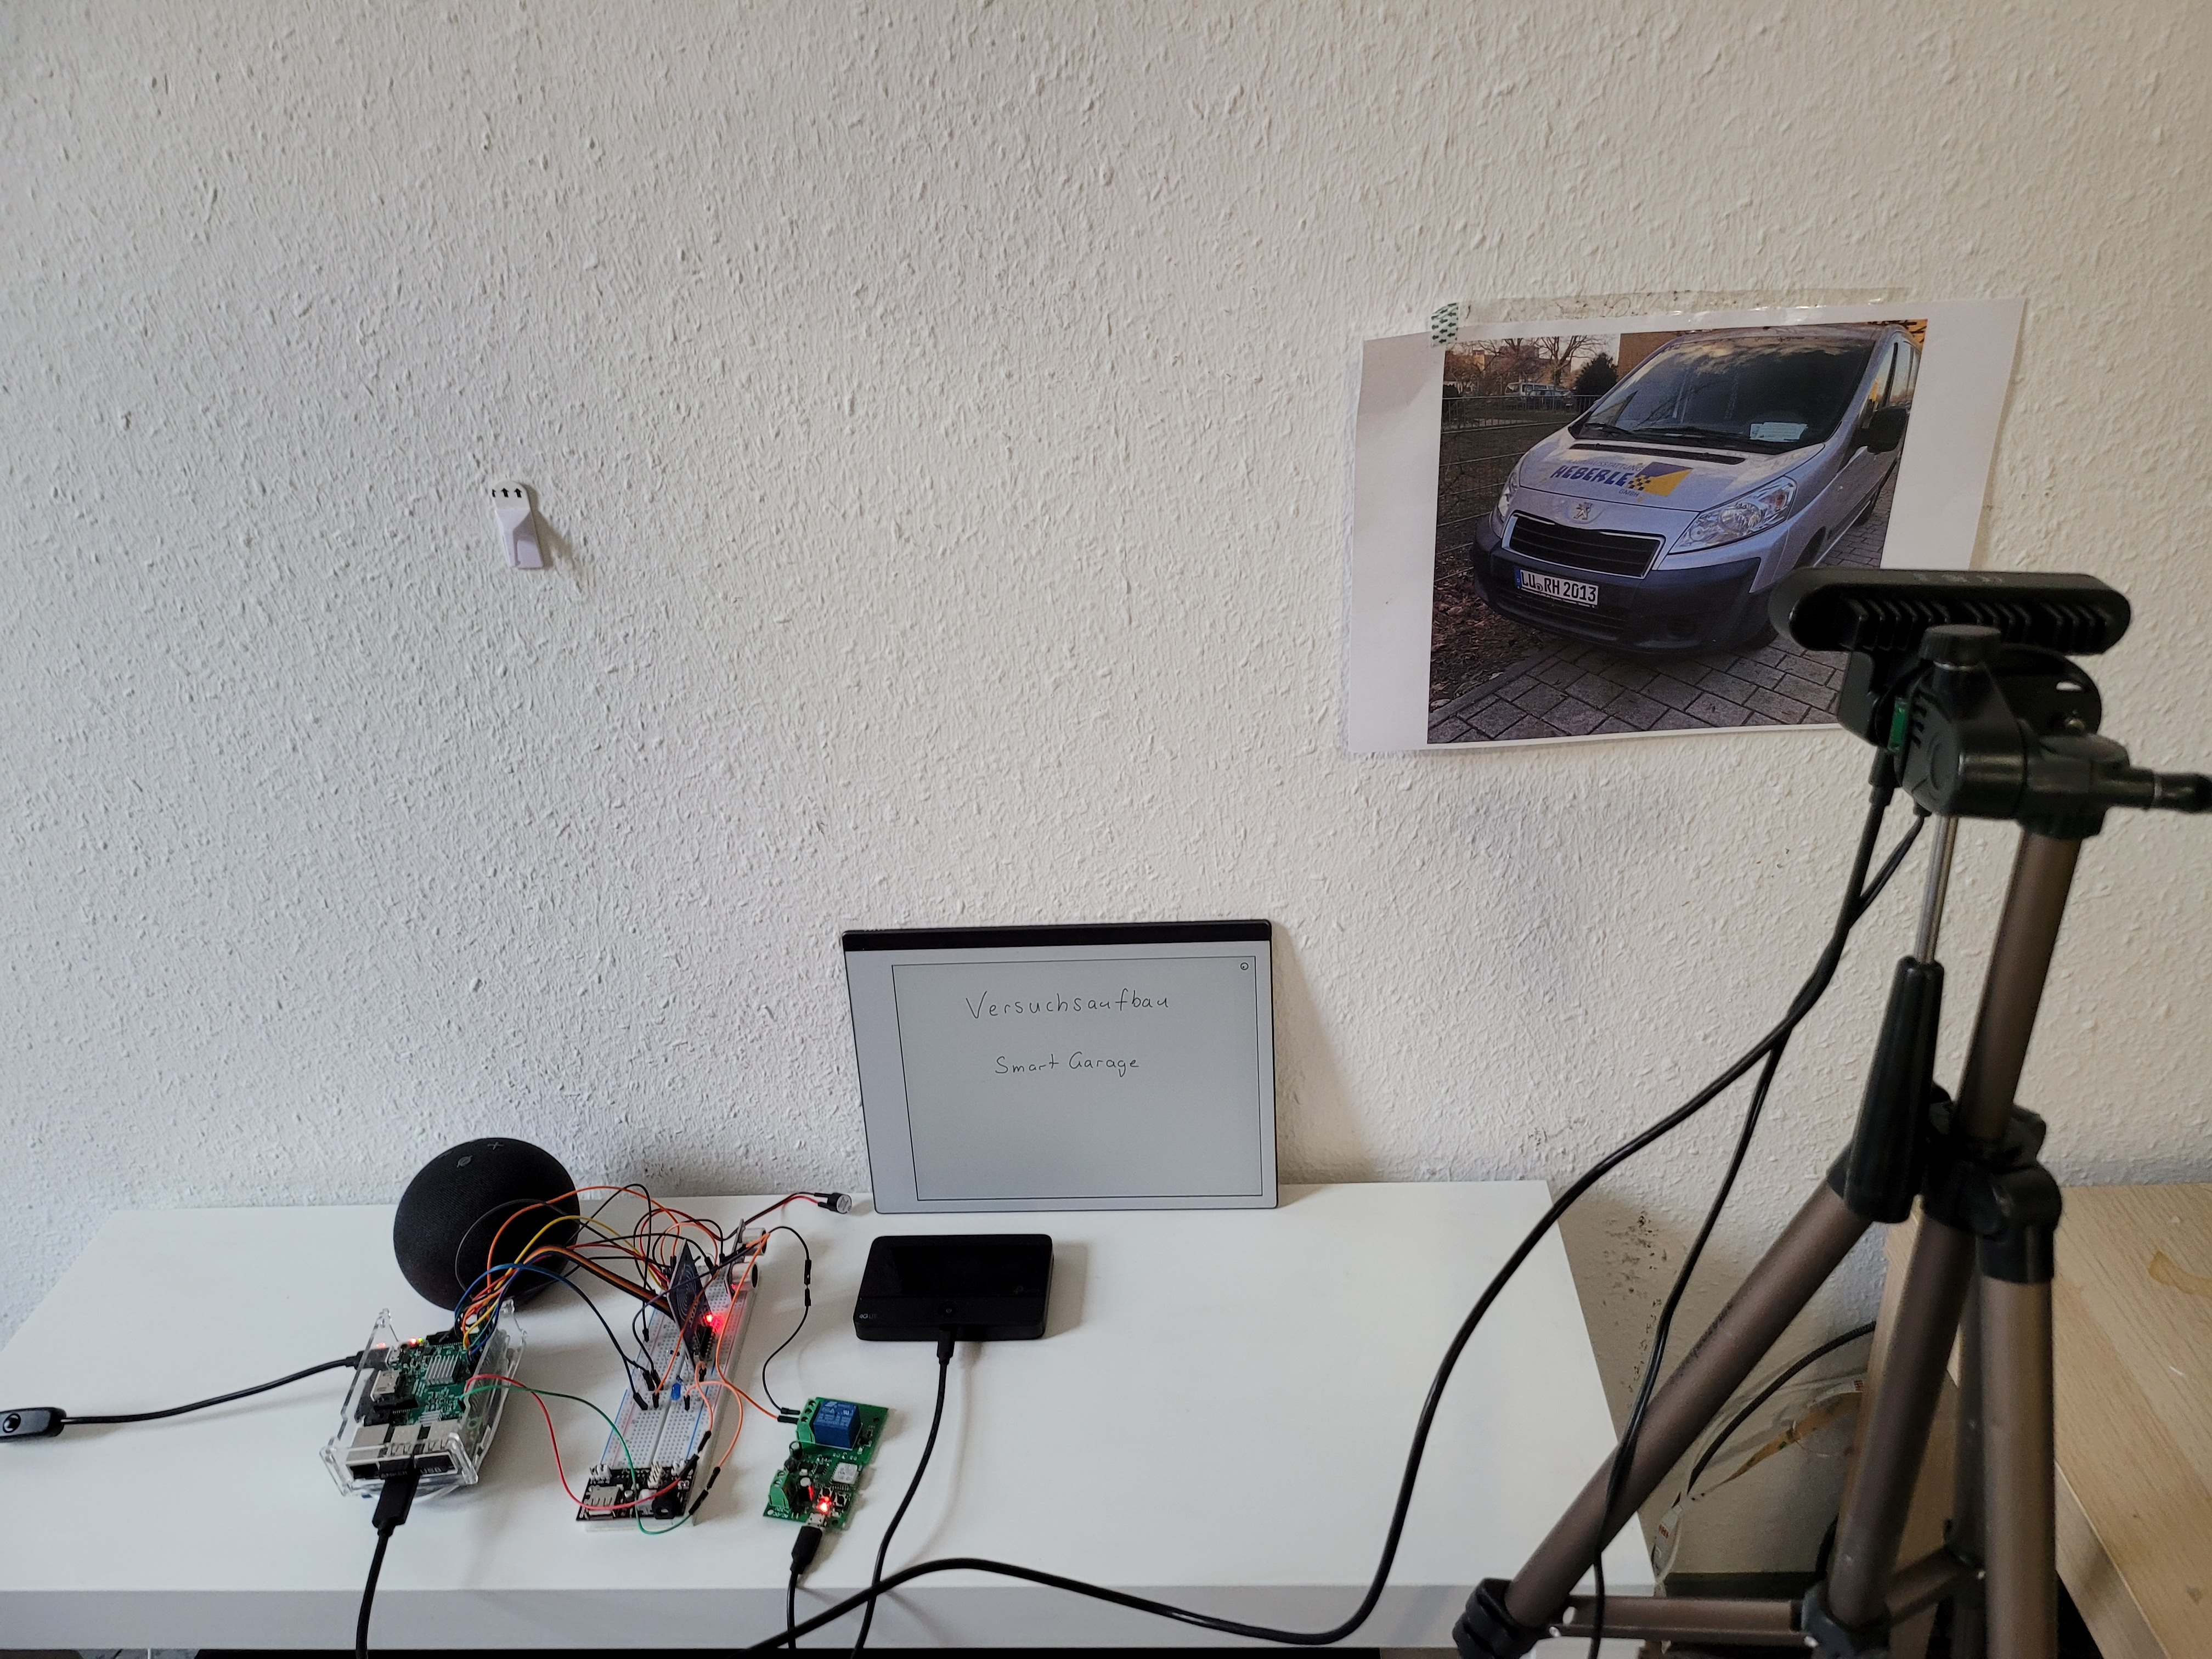
\includegraphics[scale=0.08]{\imagedir/Foto (2).jpg}
	\captionsetup{format=hang}
	\caption[Foto Aufbau 2]{\label{Aufbauanhang}Aufbau mit Kamera \\Quelle: Eigene Darstellung}
\end{figure}
\begin{figure}
	\centering 
	\label{Aufbau3}
	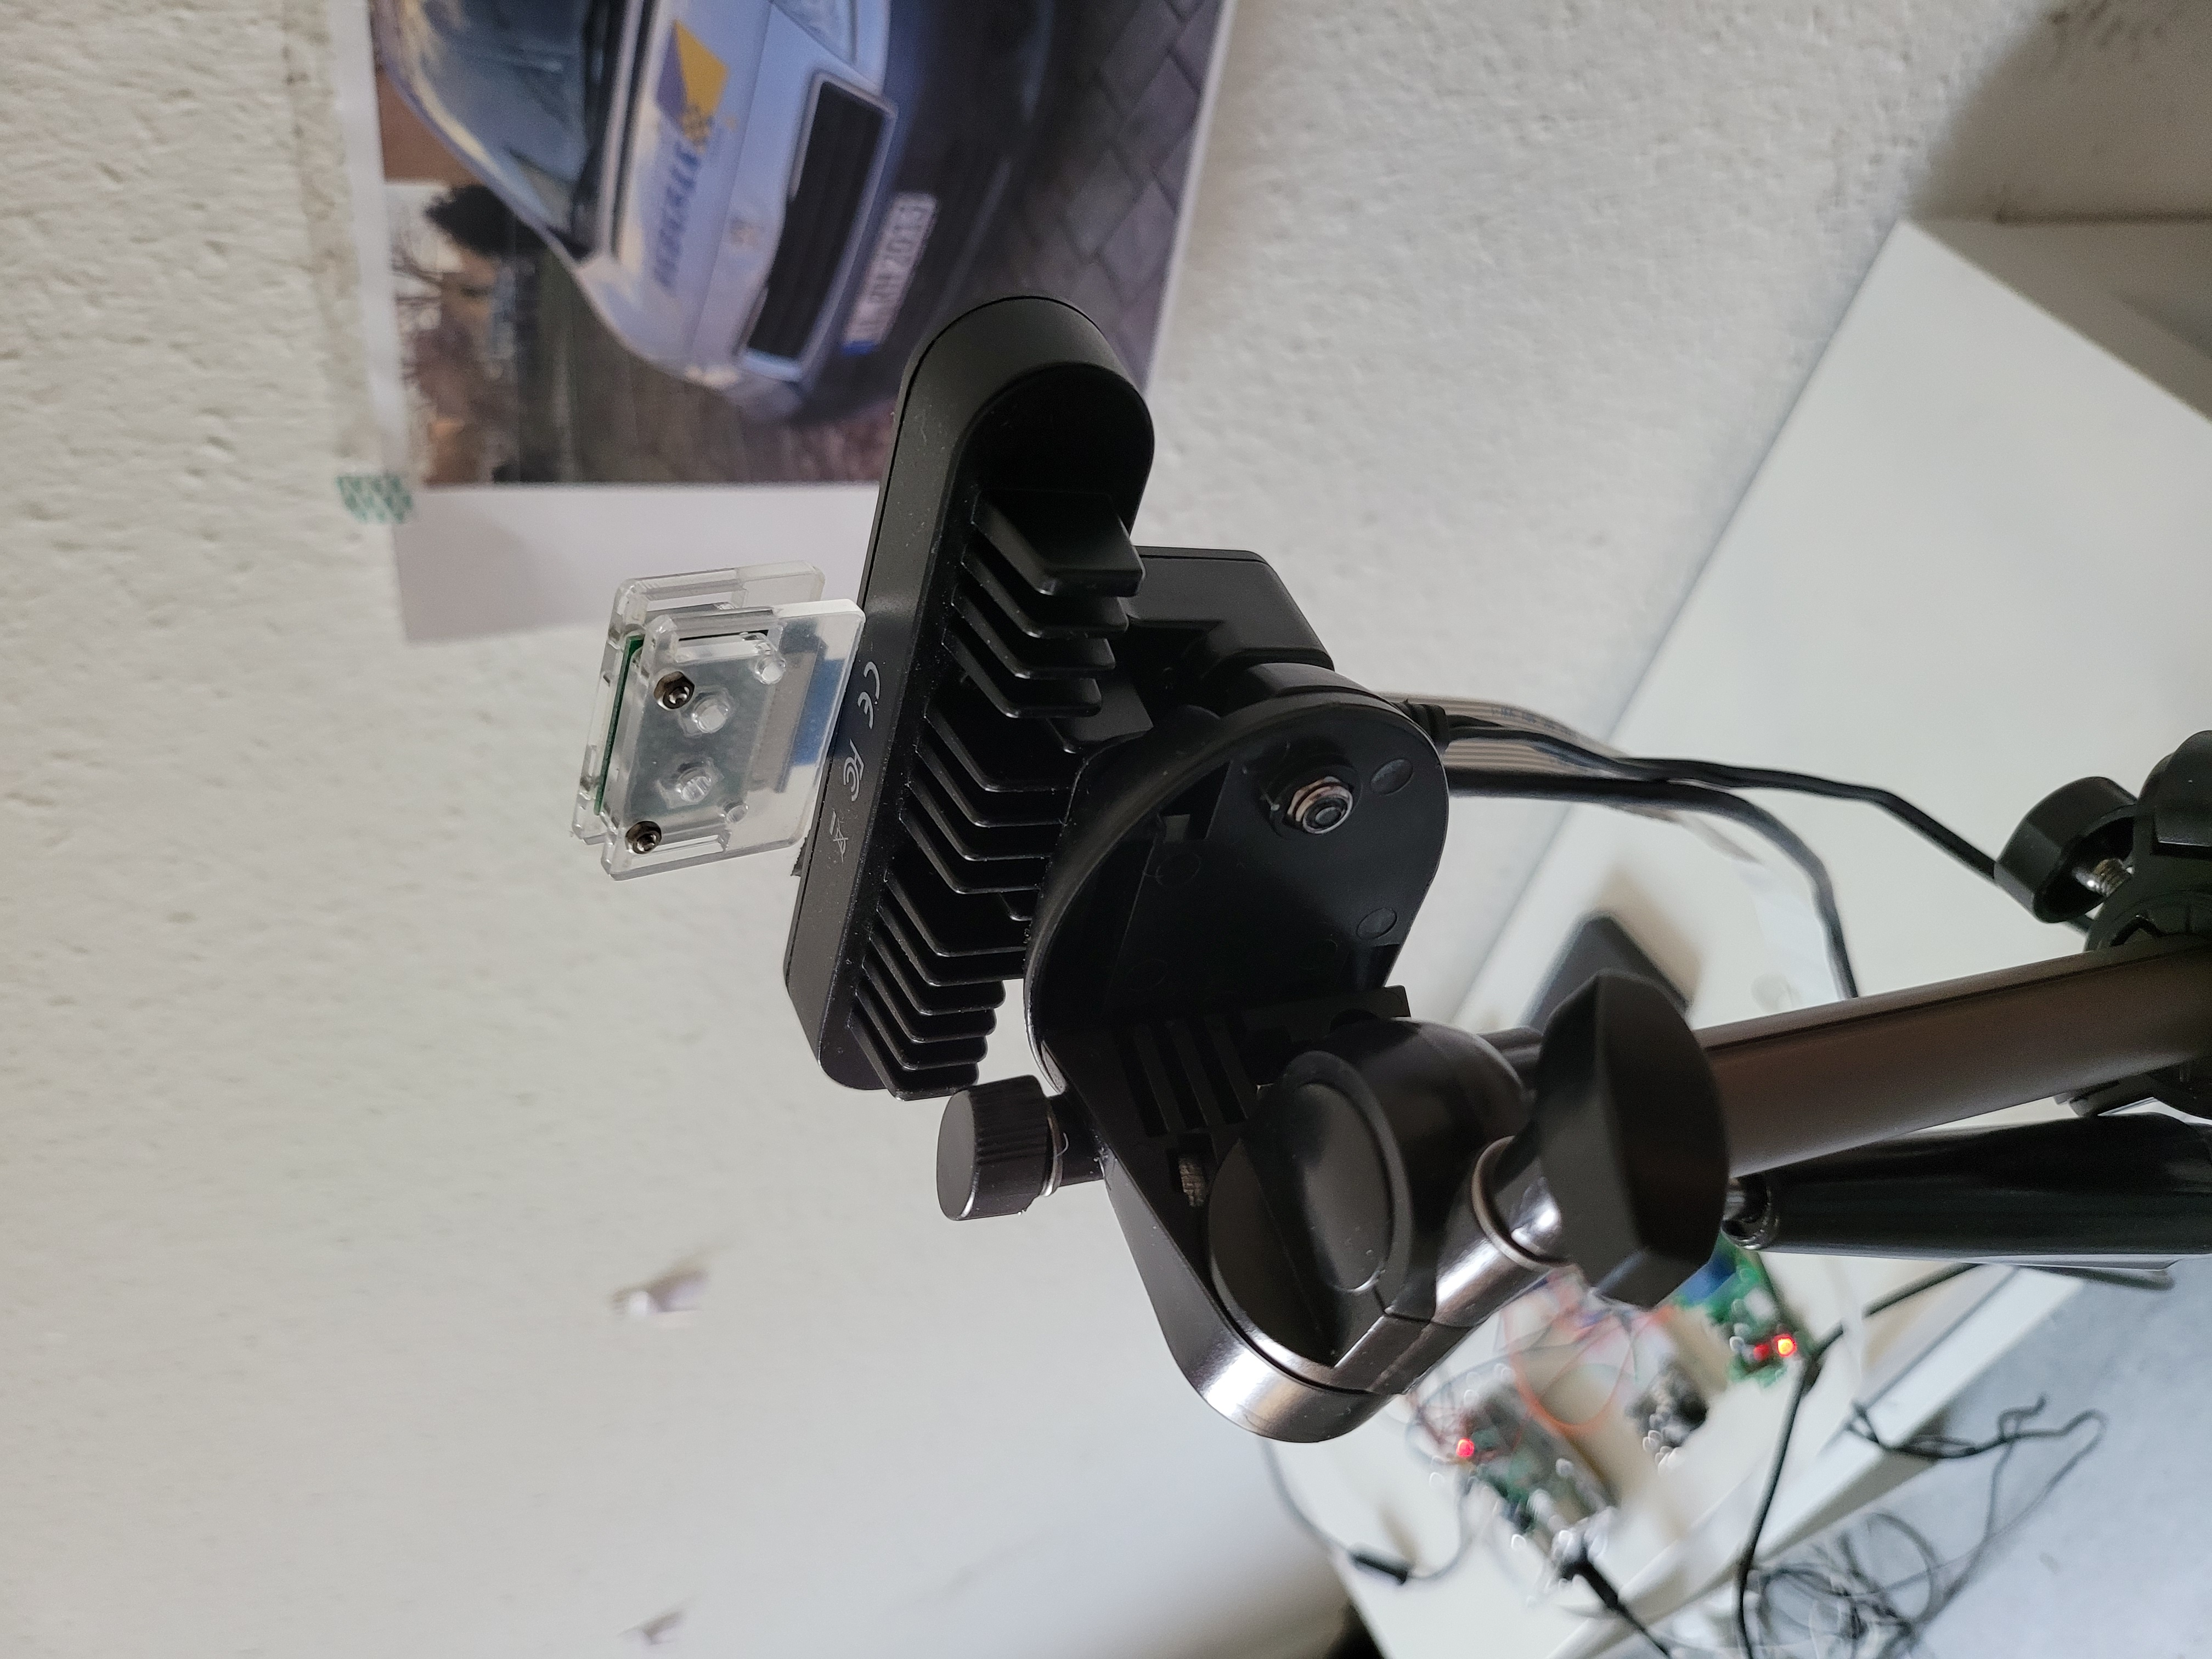
\includegraphics[scale=0.08]{\imagedir/Foto (3).jpg}
	\captionsetup{format=hang}
	\caption[Foto Aufbau 3]{\label{}Notlösung mit Raspi-Kamera nach Defekt \\Quelle: Eigene Darstellung}
\end{figure}
%\begin{figure}
%	\centering 
%	\label{Aufbau4}
%	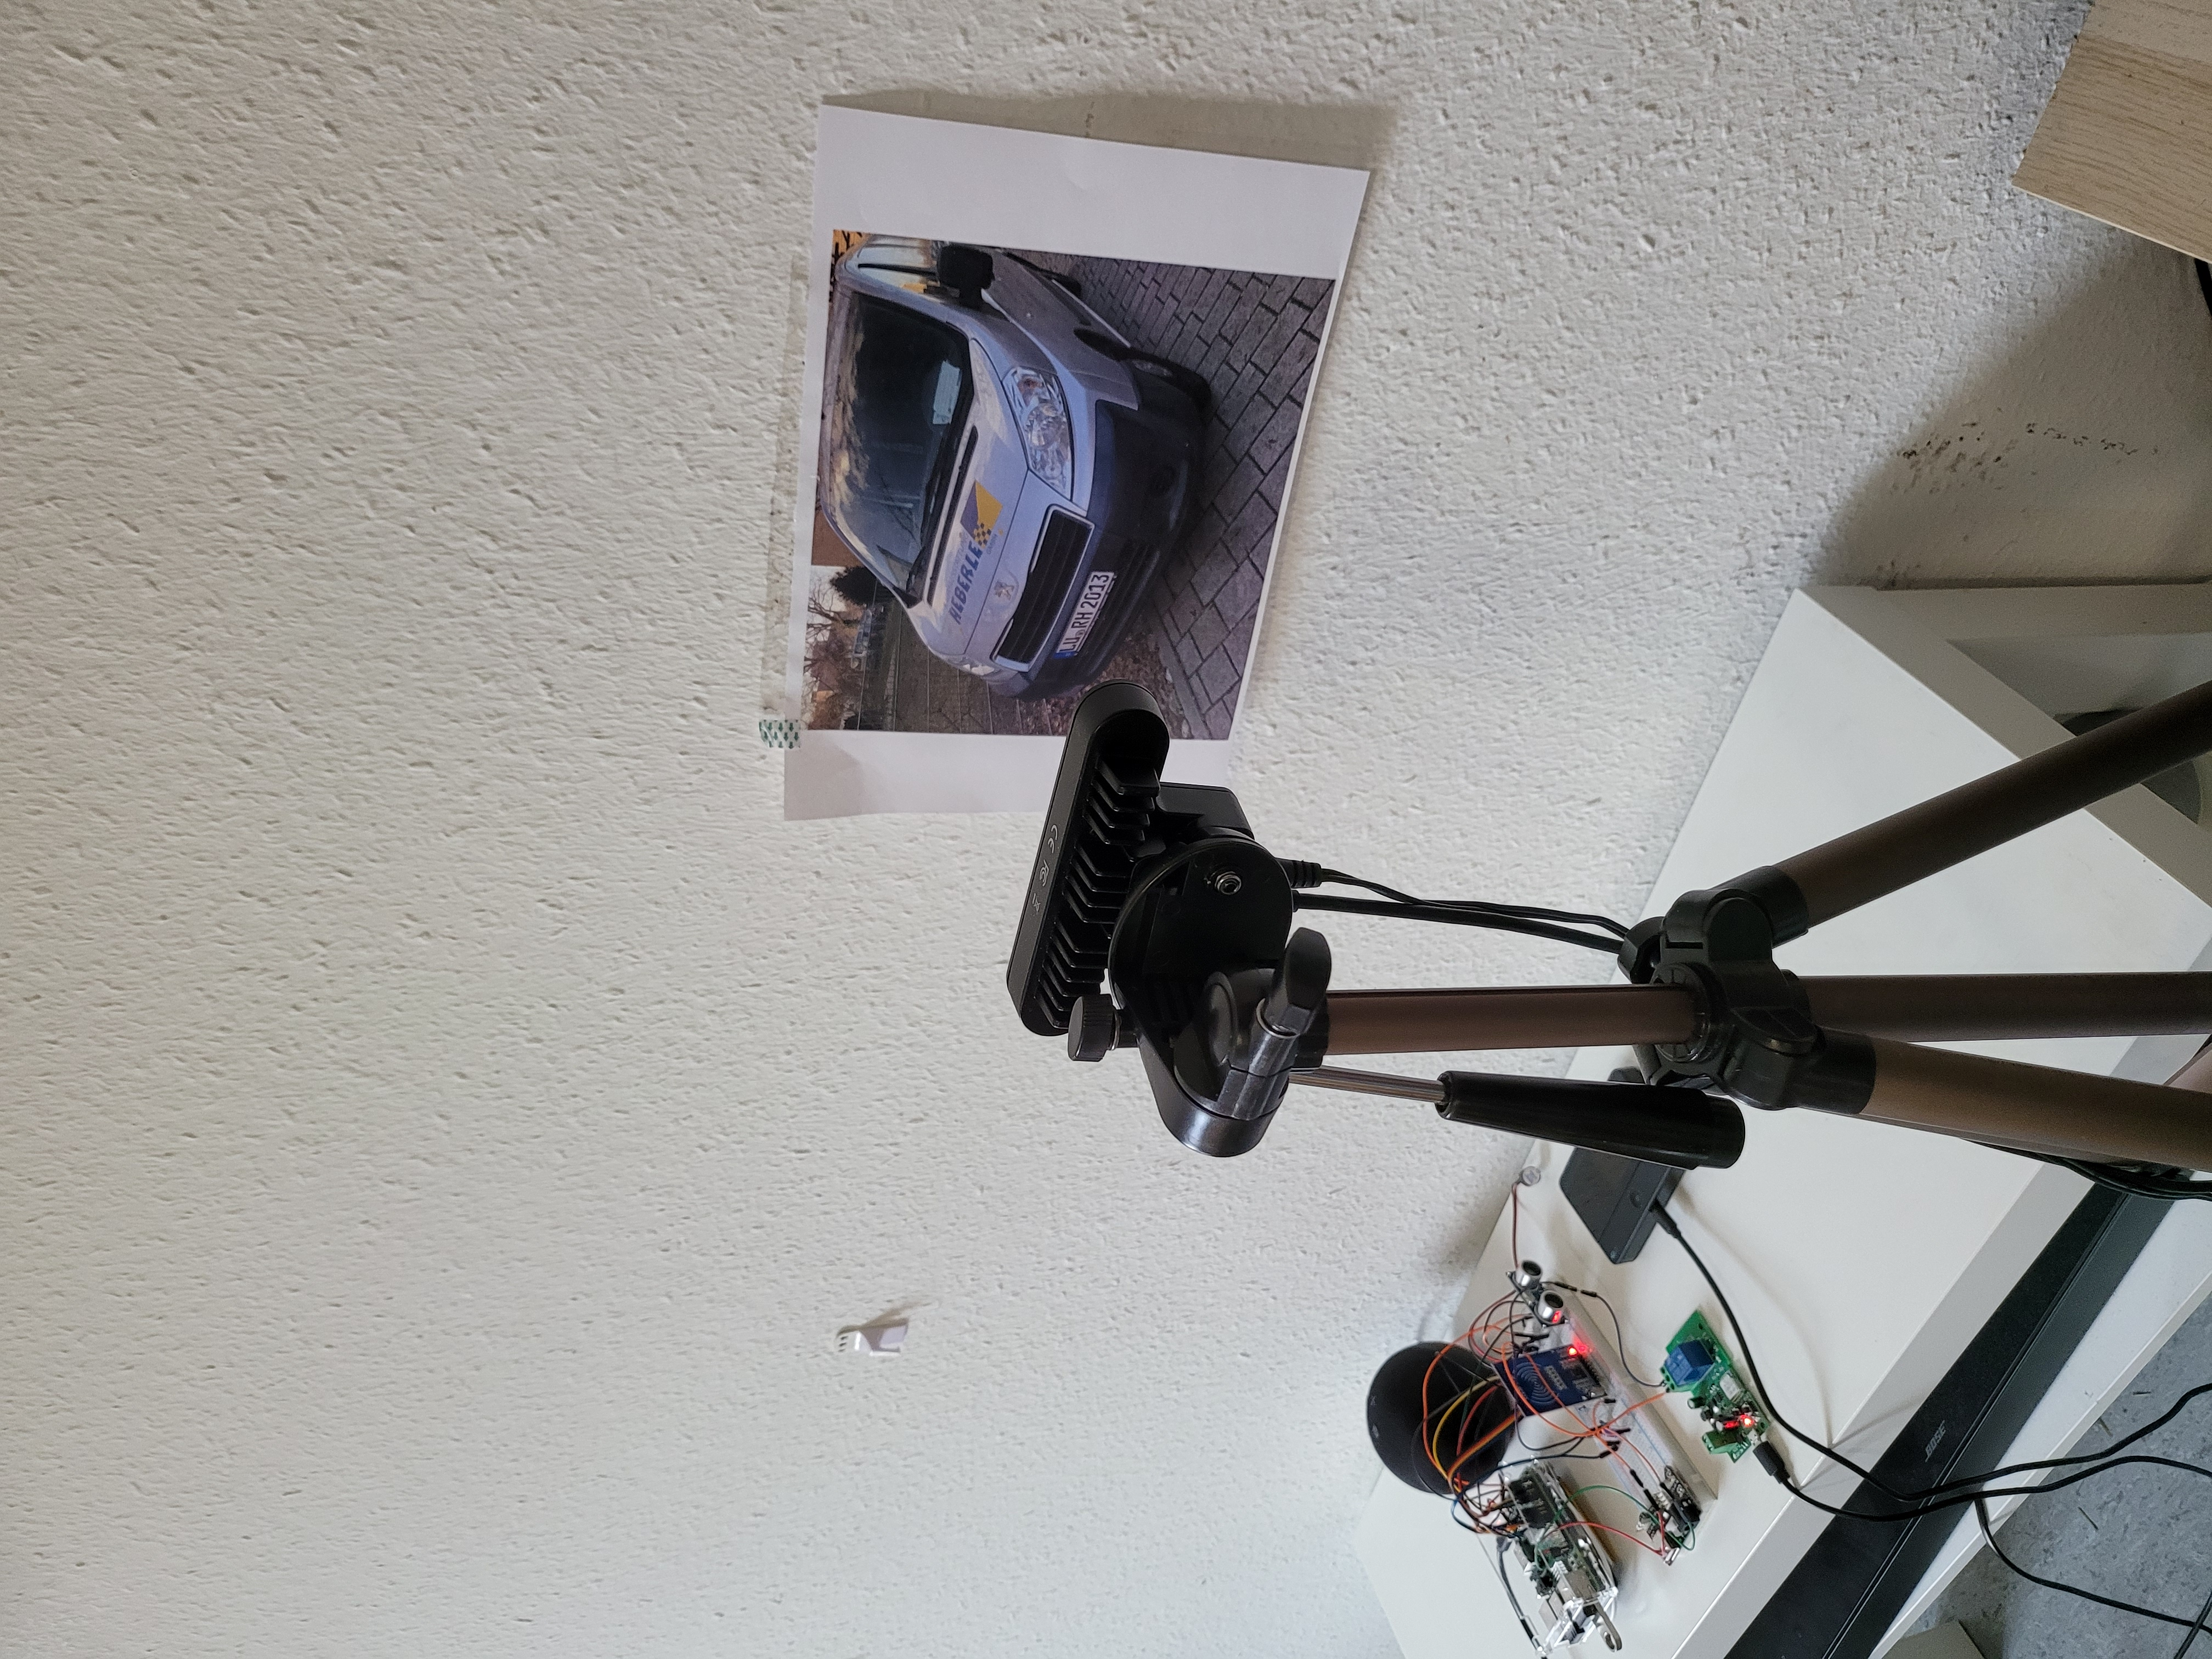
\includegraphics[scale=0.08]{\imagedir/Foto (5).jpg}
%	\captionsetup{format=hang}
%	\caption[Steckplan]{\label{}Steckplan der gesamten Hardware \\Quelle: Eigene Darstellung}
%\end{figure}
\chapter{Fehlermeldungen}
\begin{figure}[h]
	\centering
	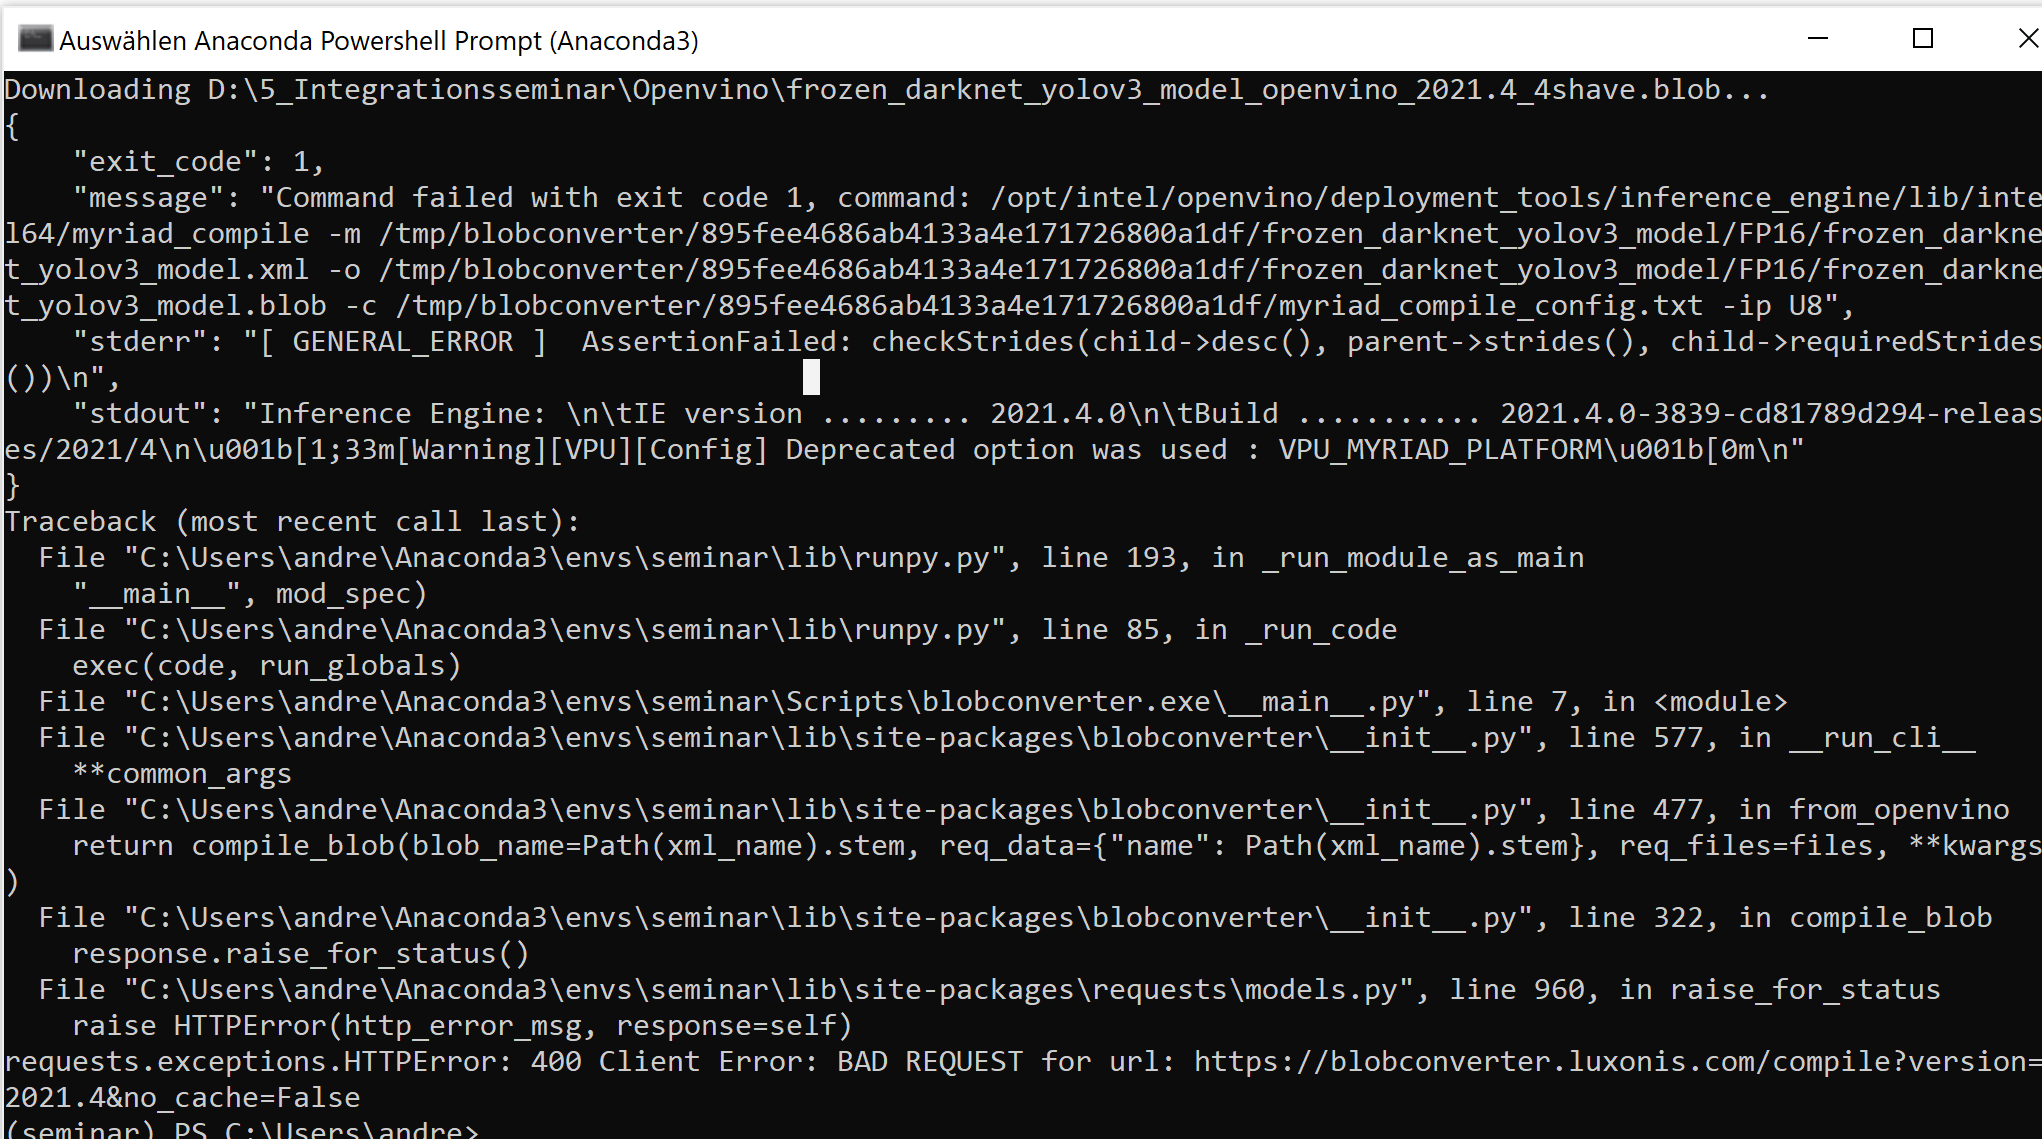
\includegraphics[width=0.9\linewidth]{img/Fehler}
	\caption[Fehlermeldung Blobkonvertierung]{Fehlermeldung beim Konvertieren des Darknet-Blobfiles}
	\label{Fehler}
\end{figure}



%% !TEX root =  master.tex
\chapter{Beispiel-Anhang: Noch ein Testanhang}
nochmal: lipsum ...

%%%%%%%%%%%%%%%%%%%%%%%%%%%%%%%%%%%

\singlespacing

%%%%%%%%%%%%%%%%%%%%%%%%%%%%%%%%%%%
% LITERATURVERZEICHNIS
% @stud: Literaturverzeichnis in Datei bibliography.bib anpassen. 
%
% Alternative zu Verwendung von \initializeBibliography: Citavi ...
% (dann \initializeBibliography auskommentieren und eigenes LaTex Coding verwenden)
%
\initializeBibliography
%%%%%%%%%%%%%%%%%%%%%%%%%%%%%%%%%%%

%%%%%%%%%%%%%%%%%%%%%%%%%%%%%%%%%%%
% INDEX
% @stud: ggf. Index auskommentieren, wenn nicht benötigt
%
\addcontentsline{toc}{chapter}{Index}
\printindex

\end{document}
